% -----------------------------------------------------------------------------
% 1) Introduce toy percolation model
% 2) Include stochastic infectivity parameter
% 3) Show behaviour in one and two dimensions
% 4) Set the basis model and establish the main ensemble method 
% -----------------------------------------------------------------------------

\chapter{Tree disease: a simple lattice model}
\label{chapter:SLM}
% 1. emphasis generality
% 2. emphasis the simplicity 
% 3. the vale in this chapter is ?
Typically, models of tree disease are complicated and involve multiple parameters informed by experimental data. Furthermore, modelling a specific pathosystem requires in-depth, specialist knowledge to incorporate biological realism, such as pathogen lifecycles or environmental suitability. This chapter shall outline a model of tree disease, beginning from simplicity, that will lay the foundations for more detailed treatment in later chapters.
Consequently, the compartmentalised $SIR$, percolation-based, model used by \cite{OROZCOFUENTES201912} will be recounted. 
From first principles, this involves an analysis of one parameter, tree density $\rho$, leading to a mathematical and conceptual definition of percolation. 
The simple one-parameter model will then give way to a discussion of criticality and self-similarity in the context of tree-based epidemics. 
The discussion will include a summary of critical phenomena and some universal behaviour within the model.
Crucially, this this chapter demonstrates the importance of thresholds in the spread of tree-based diseases.

Having established a simple one-parameter model, a more involved two-parameter, `stochastic percolation', model, will be developed and examined. 
Stochastic percolation will include an extra parameter representing the degree of pathogen infectivity. 
In general, measuring infectivity is challenging and subject to much spatial and temporal variation, such as changing climatic/environment conditions or species-level genetic variations in susceptibilities.  
However, including a stochastic infectivity parameter is essential to construct representative models of tree-based epidemics. 
In particular to tree disease, the susceptibility and infectivity between trees are thought to vary widely over a landscape. 
The two-parameter model will constitute a simple lattice model (SLM) of disease dynamics. This introductory chapter will introduce an ensemble-averaging method used throughout the thesis. 
In the present case, this takes the form of an investigation into the SLM behaviour, using ensemble-averaged parameter sweeps.

Lastly, the results of early-warning signals (EWS), investigated by \cite{OROZCOFUENTES201912}, will be extended. 
Extensions will include forming an alternate lattice configuration and a metric that permits clearer EWS detection. %
Additionally, EWS are generalised to a two-dimensional parameter-space of $\rho$ and $\beta$ from which follows the observation that it is easier to observe EWS through specific parameter combinations.

\section{Percolation theory\textemdash formalism}
% understand universality class and scaling exponents 
% we consider small timescales and neglect regrowth factors
We begin with a square lattice $\mathbb{L}$ in two dimensions, each site in the lattice can be in one of two states: %
open with probability $\rho$ or closed with probability ($1-\rho$). %
The probability $\rho$ therefore describes a density parameter and encapsulates the occupancy of a random % JS avoid using "random". Describe as a distribution (eg a gamma distribution?) 
homogeneous distribution of open and closed lattice positions. %
One open site ($c_p$) is connected to another ($c_q$) if laid within the Von Neumann neighbourhood \cite{toffoli1987cellular}. %
% \citep[see][p 50]{toffoli1987cellular}.
A connected set of open nearest neighbours define a cluster denoted by $C$, where $c_i \in C$.%
Given the set $C$, it is possible to traverse between any member site $c_i \in C$ by moving through the lattice in either horizontal or vertical steps `Von Neumann motion'. %
Given two distinct non-overlapping clusters $c_i \in C_1$ and $c_j \in C_2$, then $c_i \neq c_j $ i.e. there is no way to jump from $C_1$ to $C_2$ following Von Neumann motion. %
Connectivity is defined between lattice sites rather than the edges which connect them. %
This is known as `site' percolation\textemdash opposed to `bond' percolation. %

If $\rho$ is close to zero, only very small clusters would be present (as a disordered system), %
conversely, if $\rho$ is large then one very large connected network of open positions would dominate the domain (an ordered system). %
At some point for $\rho \in [0, 1]$ a critical threshold ($\rho_c$) would be reached and a singularity of connected open lattice positions would span the length of an infinite sized lattice. %
On a finite lattice, the cluster is said to percolate and form a `spanning cluster' ($C_\infty$) that extends between at least two different edges of the lattice. %
The formation of the spanning cluster occurs abruptly between a very narrow range of $\rho$ values. %
Therefore, the threshold for percolation defines a critical-point \cite{STAUFFER19791}. %

The critical point can be defined as the least value of $\rho$ where percolation occurs with non-zero probability. %
This can be formalised by first considering the probability function: $\theta (\rho)= \lbrace \rho:|C|=\infty\rbrace$ where $\theta(\rho)$ is the probability of an arbitrary site, %
within a lattice of density $\rho$, belonging to cluster $C$ of size $\infty$ (i.e. the spanning cluster). %
The critical value then satisfies: %
\begin{equation}
\label{eq:critical_threshold_1d}
    \rho _{c}=sup \lbrace \rho : \theta (\rho ) = 0 \rbrace
\end{equation}

At this point, the spanning cluster has been described conceptually. %
However, a  many nuances and technicalities complicate this given simple definition. %
For example, the probability of percolation has a non-trivial dependence on the size of the lattice. %
If the mean cluster size, defined by a `characteristic' cluster length $C_r$, is above or comparable to $L$, then the percolation could be observed despite the density residing in the sub-critical regime. %
The size of the lattice $\mathbb{L}$ is therefore required to be sufficiently large, compared to individual lattice positions (or microscopic interactions) in order to reliably approximate the true threshold $\rho_c$ and spanning cluster $C_{\infty}$. %
When this is true, the results will be insensitive to small changes in $L$ and the threshold $\rho_c$ will remain constant. %

All proceeding simulations in this thesis are conducted on finite sized domains between two and three orders of magnitude larger than individual lattice points. %
The model presented in this chapter, first published by \cite{OROZCOFUENTES201912}, was found to agree with the accepted percolation threshold, when the lattice had size $L \sim 500\times500$. %
As such, the lattice configuration used here will assume the same size-configuration. %

By intuition, it is clear to see analogies between percolation and epidemiology: open lattice positions act as susceptible members of a population ($S$) and $\rho$ defines a density of the hosts. %
In this paradigm, the spanning cluster describes a high-impact epidemic that spreads uncontrollably. %
Small-medium sized clusters (existing at or slightly below threshold) describe short-lived, failed epidemics where the pathogen spreads for a time before becoming extinct \cite{gilligan2008epidemiological}. %

These analogies have clear limitations when describing mobile hosts. %
Fortunately, trees are sessile and immobile. %
Percolation theory therefore provides a useful framework for modelling tree diseases (see Chapter \ref{section:lit-rev-perc} for a review of percolation-based epidemiological models). %
Forming a percolation-based lattice model of tree disease requires us to first combine a compartmental $SIR$-like model within the aforementioned lattice $L$. %
Additionally, an appropriate transmission dynamic is needed to model the spread of disease between lattice points. %


\section{Percolation-based $SIR$ toy model}

A rational toy model of tree disease can now be outlined in good conscience. % JS_rational here mean information-based
The density $\rho$ is re-interpreted as the probability of a susceptible tree $S$ (given a numerical value $1$) and empty lattice positions to define an insusceptible state $\emptyset$ (with numerical value $0$). %
If a susceptible tree neighbours an infected tree, the disease  will transition into the $I$ compartment (having a numerical value of $2$) with a probability of 1.0. %
The neighbourhood being defined by the Von-Neumann neighbourhood. %
After an arbitrary number of time-steps $T$ an infected tree will die and transition into the removed state $R$, see appendix \ref{a:propagation} for more information on how this is implemented computationally. %
For simplicity, the infectious life-time will not be considered as a parameter but will remain fixed at $T=1.0$, %
this will be revisited in section \ref{ch3:two-param-model}.

At time $t=0$, a small patch lattice sites (of size $5\times5$) about the origin $L_O$ are set to occupy the infected state. %
Percolation is defined from the lattice epicenter (or origin) and is registered when a connected cluster of infectious-removed trees extend from $L_O$ to any of the four lattice boundaries. %
Each time-step through the simulation represent an arbitrary unit of time\footnote{For individual trees this is typically of the order of years.} %
and the disease propagates according to the spreading heuristics. %
The numerical simulations then terminates if one of three boundary conditions is met: %
1) a percolation is observed %
2) the pathogen becomes extinction %
3) a time-horizon of $N$ steps is reached. %
Typical simulations on a domain of size $500 \times 500$ are shown in Figure \ref{fig:ch3-perc-spread} through three time-steps. %

\begin{figure}
    \centering
    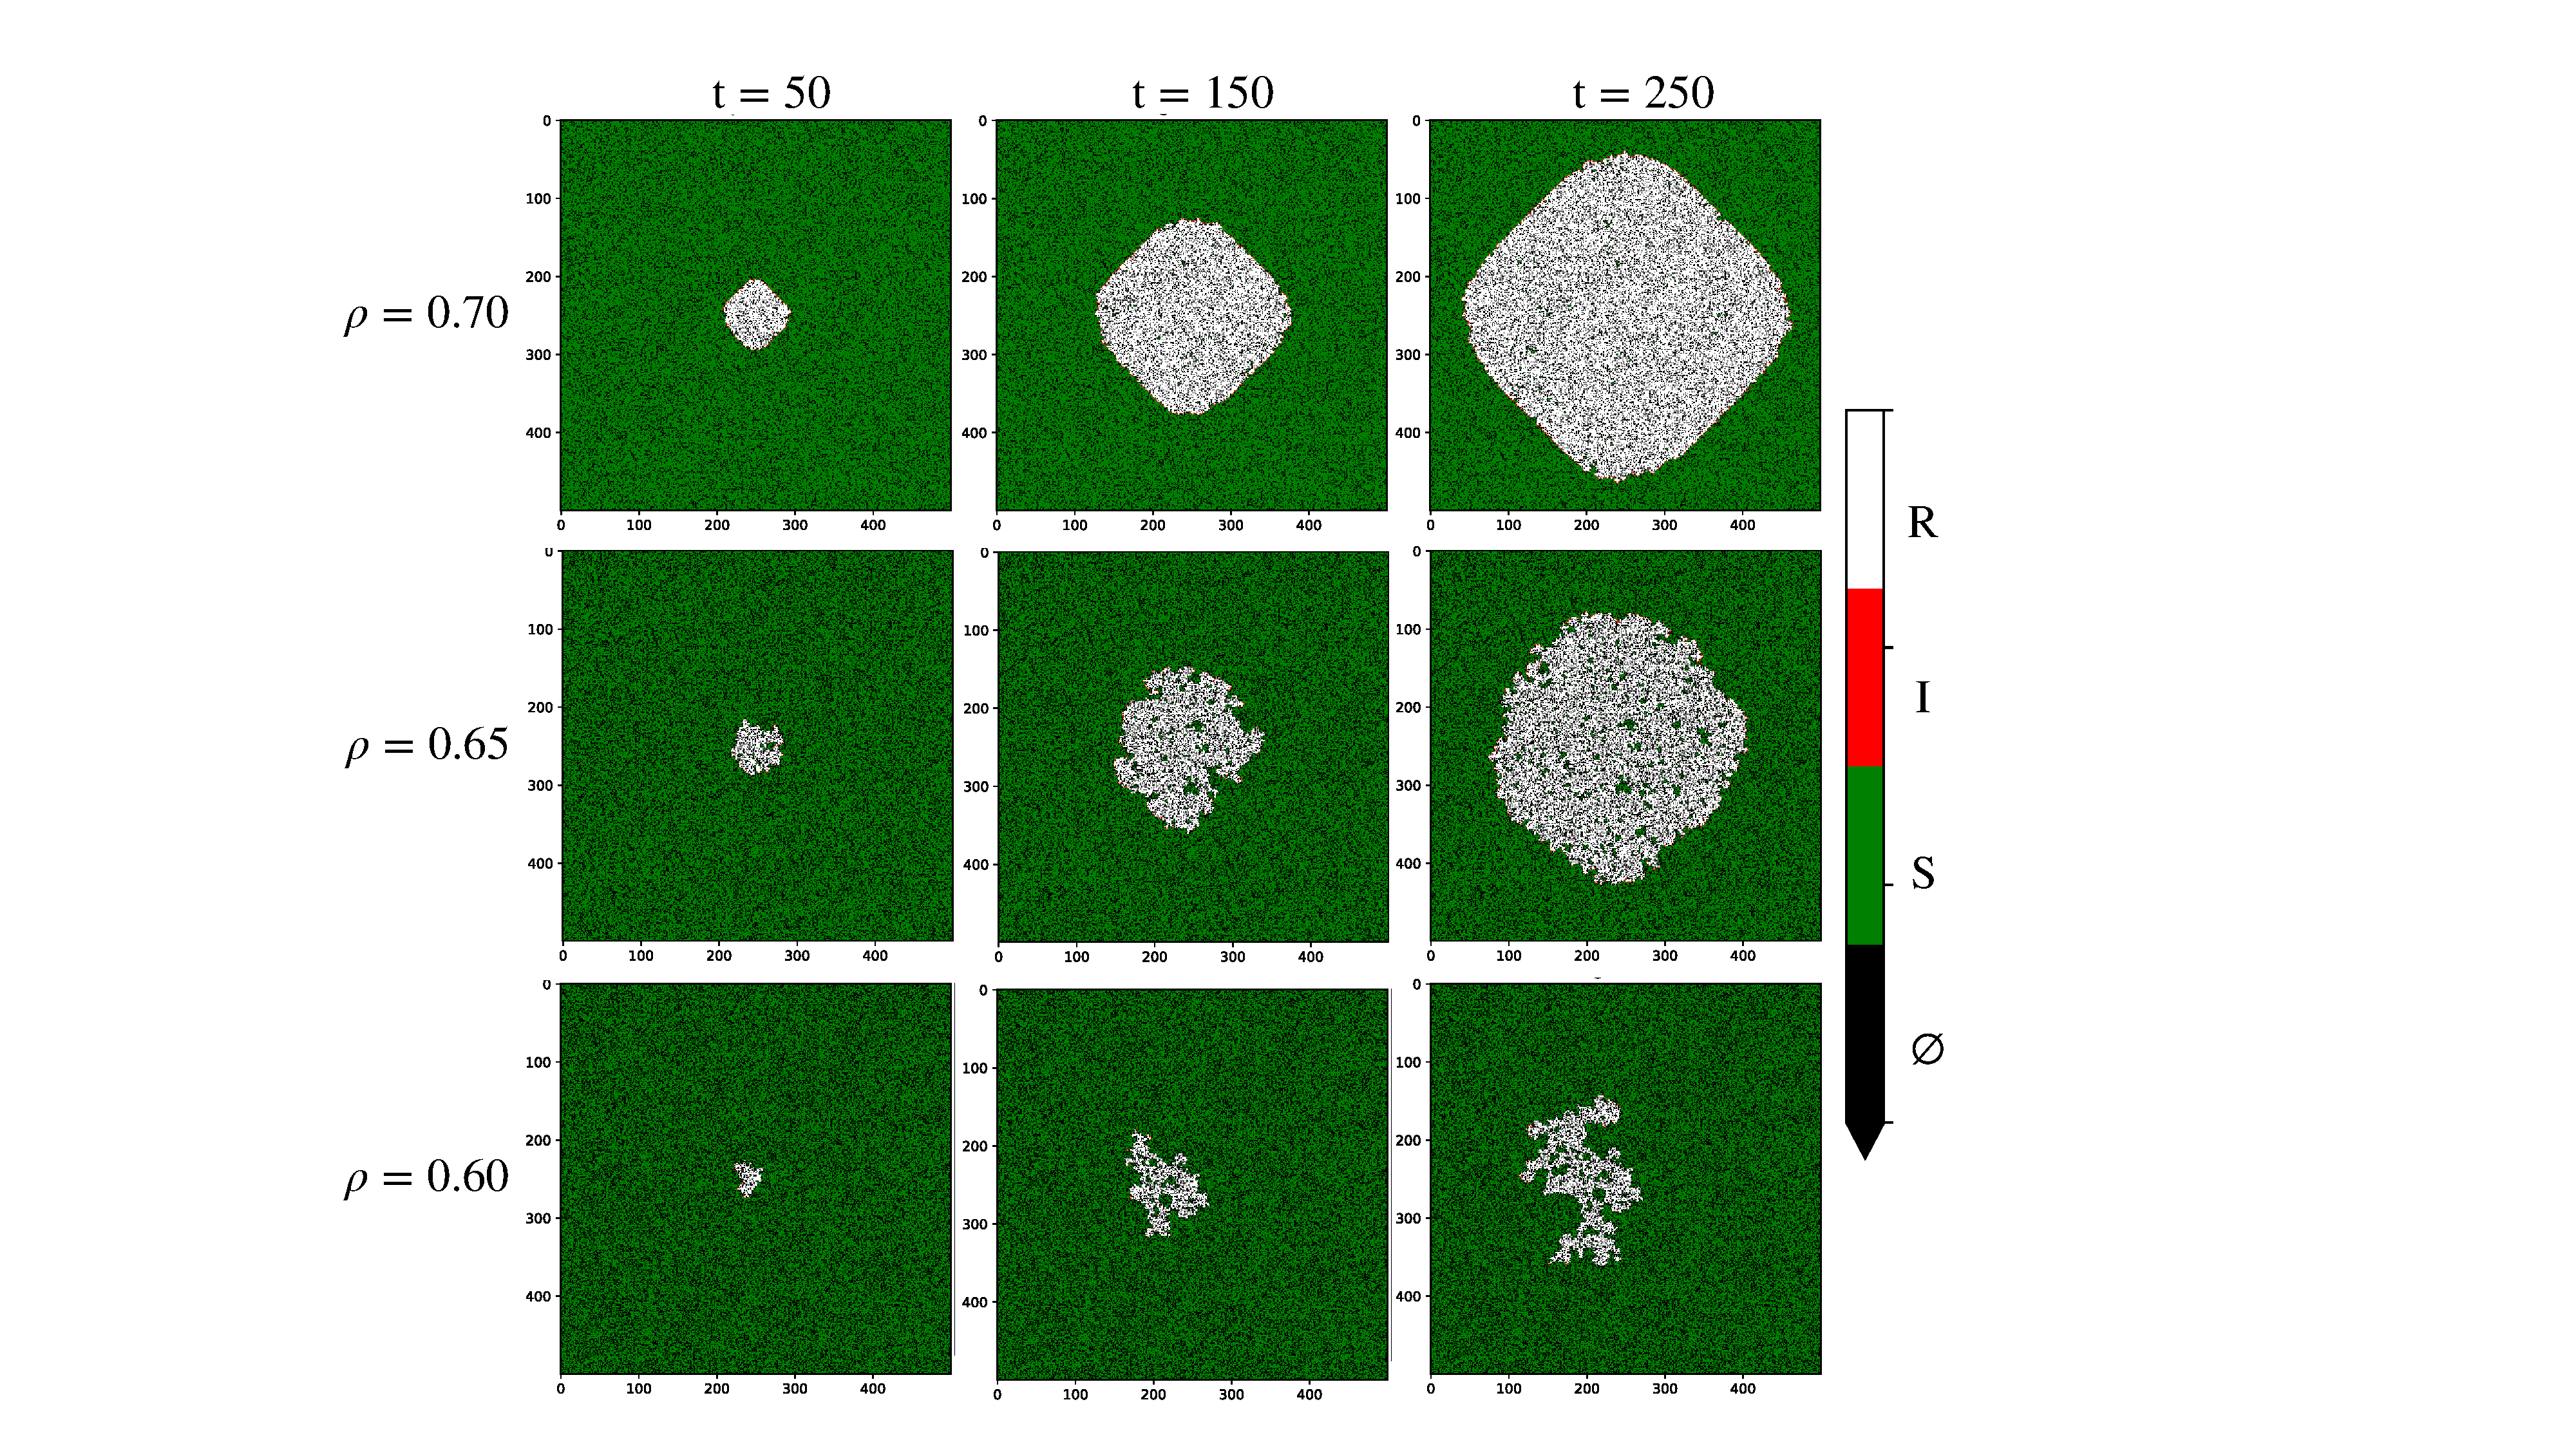
\includegraphics[scale=0.40]{chapter3/figures/figure1.pdf}
    \caption{A domain of size $\mathrm{500\times 500}$ showing the toy percolation model behaviour for three values of tree density through three successive time-steps.}
    \label{fig:ch3-perc-spread}
\end{figure}

Figure \ref{fig:ch3-perc-spread} shows dynamic simulations of disease spread through $L$. %
The first row at density $\rho=0.70$ reveals an unnatural diamond-like pattern of spread. %
This result reflects an artefact of the lattice geometry and would looks different if the lattice geometry is changed \textemdash for example, consider a triangular lattice. %
A wave-like propagation of infected trees begins to spread from the centrally-infected epicenter toward the lattice boundary. %
Later on, we shall see how the conceptual`travelling-wave' has far reaching epidemiological consequences. %
In Figure \ref{fig:ch3-perc-spread} the simulations for tree density $\rho=0.65$ begin to %
look more realistic as stochasticity within the lattice breaks up the travelling wave of infected trees into a circular front. %
For the lower density $\rho = 0.60$, the cluster of infected-removed trees begins to appear %
to be fractal-like and the pathogen wave-front interface spreads at a slower rate, %
hence traversing a smaller area. %

If an infected tree reaches the lattice boundary, the pathogen is assumed to survive and a binary value of 1 is recorded to signify percolation. %
Otherwise, a binary value of 0 is recorded for pathogen-extinction. %
Performing an ensemble of simulations and sweeping through successive values of $\rho$ allow us to ascertain the percolation threshold. %
Figure \ref{fig:ch3-perc-pr} shows the ensemble-averaged probability of percolation, $Pr(\rho)$. A critical region, between $ 0.575 < \rho_c < 0.615$, is shown in orange and separates two regimes of pathogen extinction and percolation (or epidemic). %
This is consistent with the accepted value of $0.592...$, cited in literature for a square lattice. %
 
\begin{figure}
    \centering
    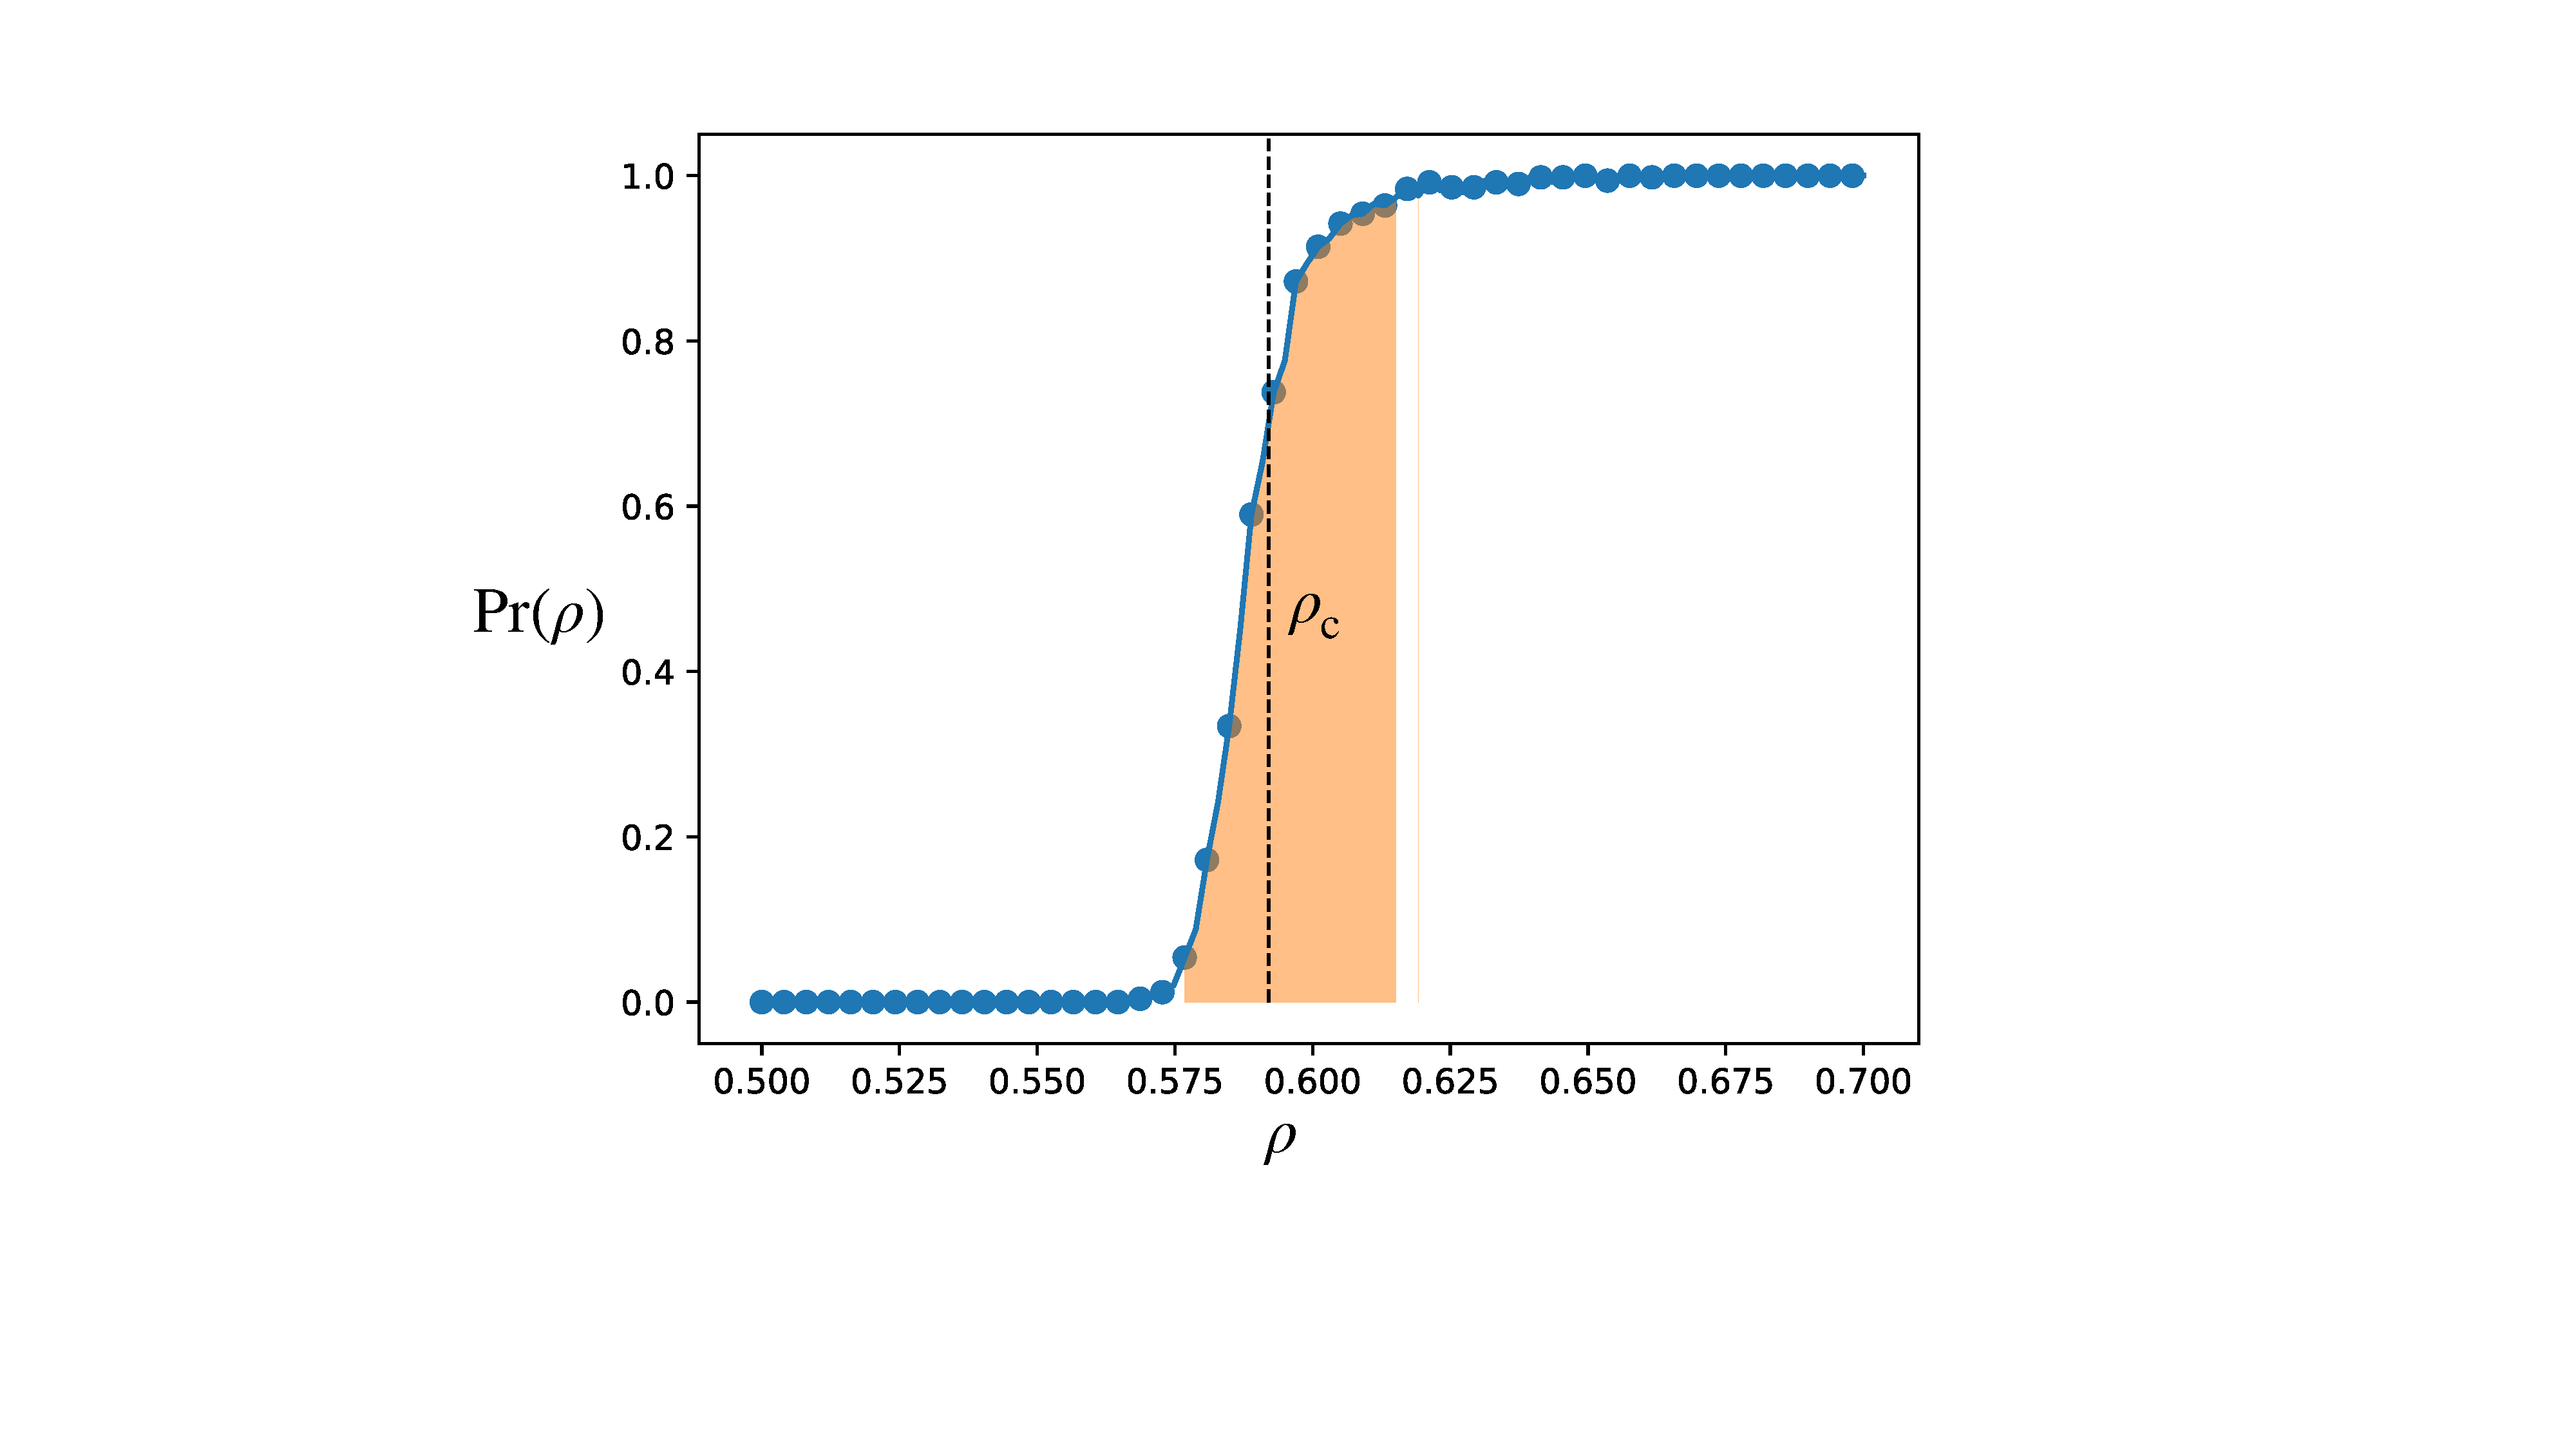
\includegraphics[scale=0.25]{chapter3/figures/figure2.pdf}
    \caption{The probability of percolation, $\mathrm{Pr(\rho)}$, determined for the toy percolation model. The critical region shown in shaded orange is consistent with classical result in percolation theory, namely $\rho_c = 0.592...$, shown by the vertical dashed line. The sharp transition between regimes has far-reaching epidemiological implications and can be likened to a threshold beyond which epidemics are possible.}
    \label{fig:ch3-perc-pr}
\end{figure}

The probability of percolation depends non-trivially on stochasticity. %
Around percolation threshold, there can be large fluctuations in the size of the clusters formed. %
Therefore, a number of repeated simulations, giving an `ensemble' \cite{gibbs1902elementary} are %
needed to be averaged in order to determine the mean of the probability distribution of percolation $Pr(\rho)$.

\subsection{Universality and criticality}
\label{section:universality}
% 1) introduce scaling laws of cluster size 
% 2) introduce fractal geometry and dependence on d i,e universality 
% 3) introduce critical scaling exponents and the form ( p - p_c )
% 4) introduce critical phenomena and phase transpositions i.e. the singularity
\begin{table}[h!]
  \begin{center}
    \begin{tabular}{l|c|c|r} % <-- Alignments: 1st column left, 2nd middle and 3rd right, with vertical lines in between
    \hline
      \textbf{Lattice} & $nn$ & \textbf{Site percolation} & \textbf{Bond percolation}\\
      \hline
      1D & 2 & 1 & 1\\
      Square 2D & 4 & 0.593 & $1/2$\\
      Triangular 2D & 6 & $1/2$ & 0.347\\
      Honeycomb & 3 & 0.696 & 0.653\\
      Diamond & 4 & 0.43 & 0.388\\
      Voronoi & - & 0.714 & 0.667\\
    \hline
    \end{tabular}
    \caption{Percolation thresholds for various lattice types showing the number of nearest neighbours $nn$ along with site and bond thresholds. Data given by \cite{stauffer2018introduction, PhysRevE.80.041101}}
    \label{tab:perc}
  \end{center}
\end{table}

\begin{figure}
    \centering
    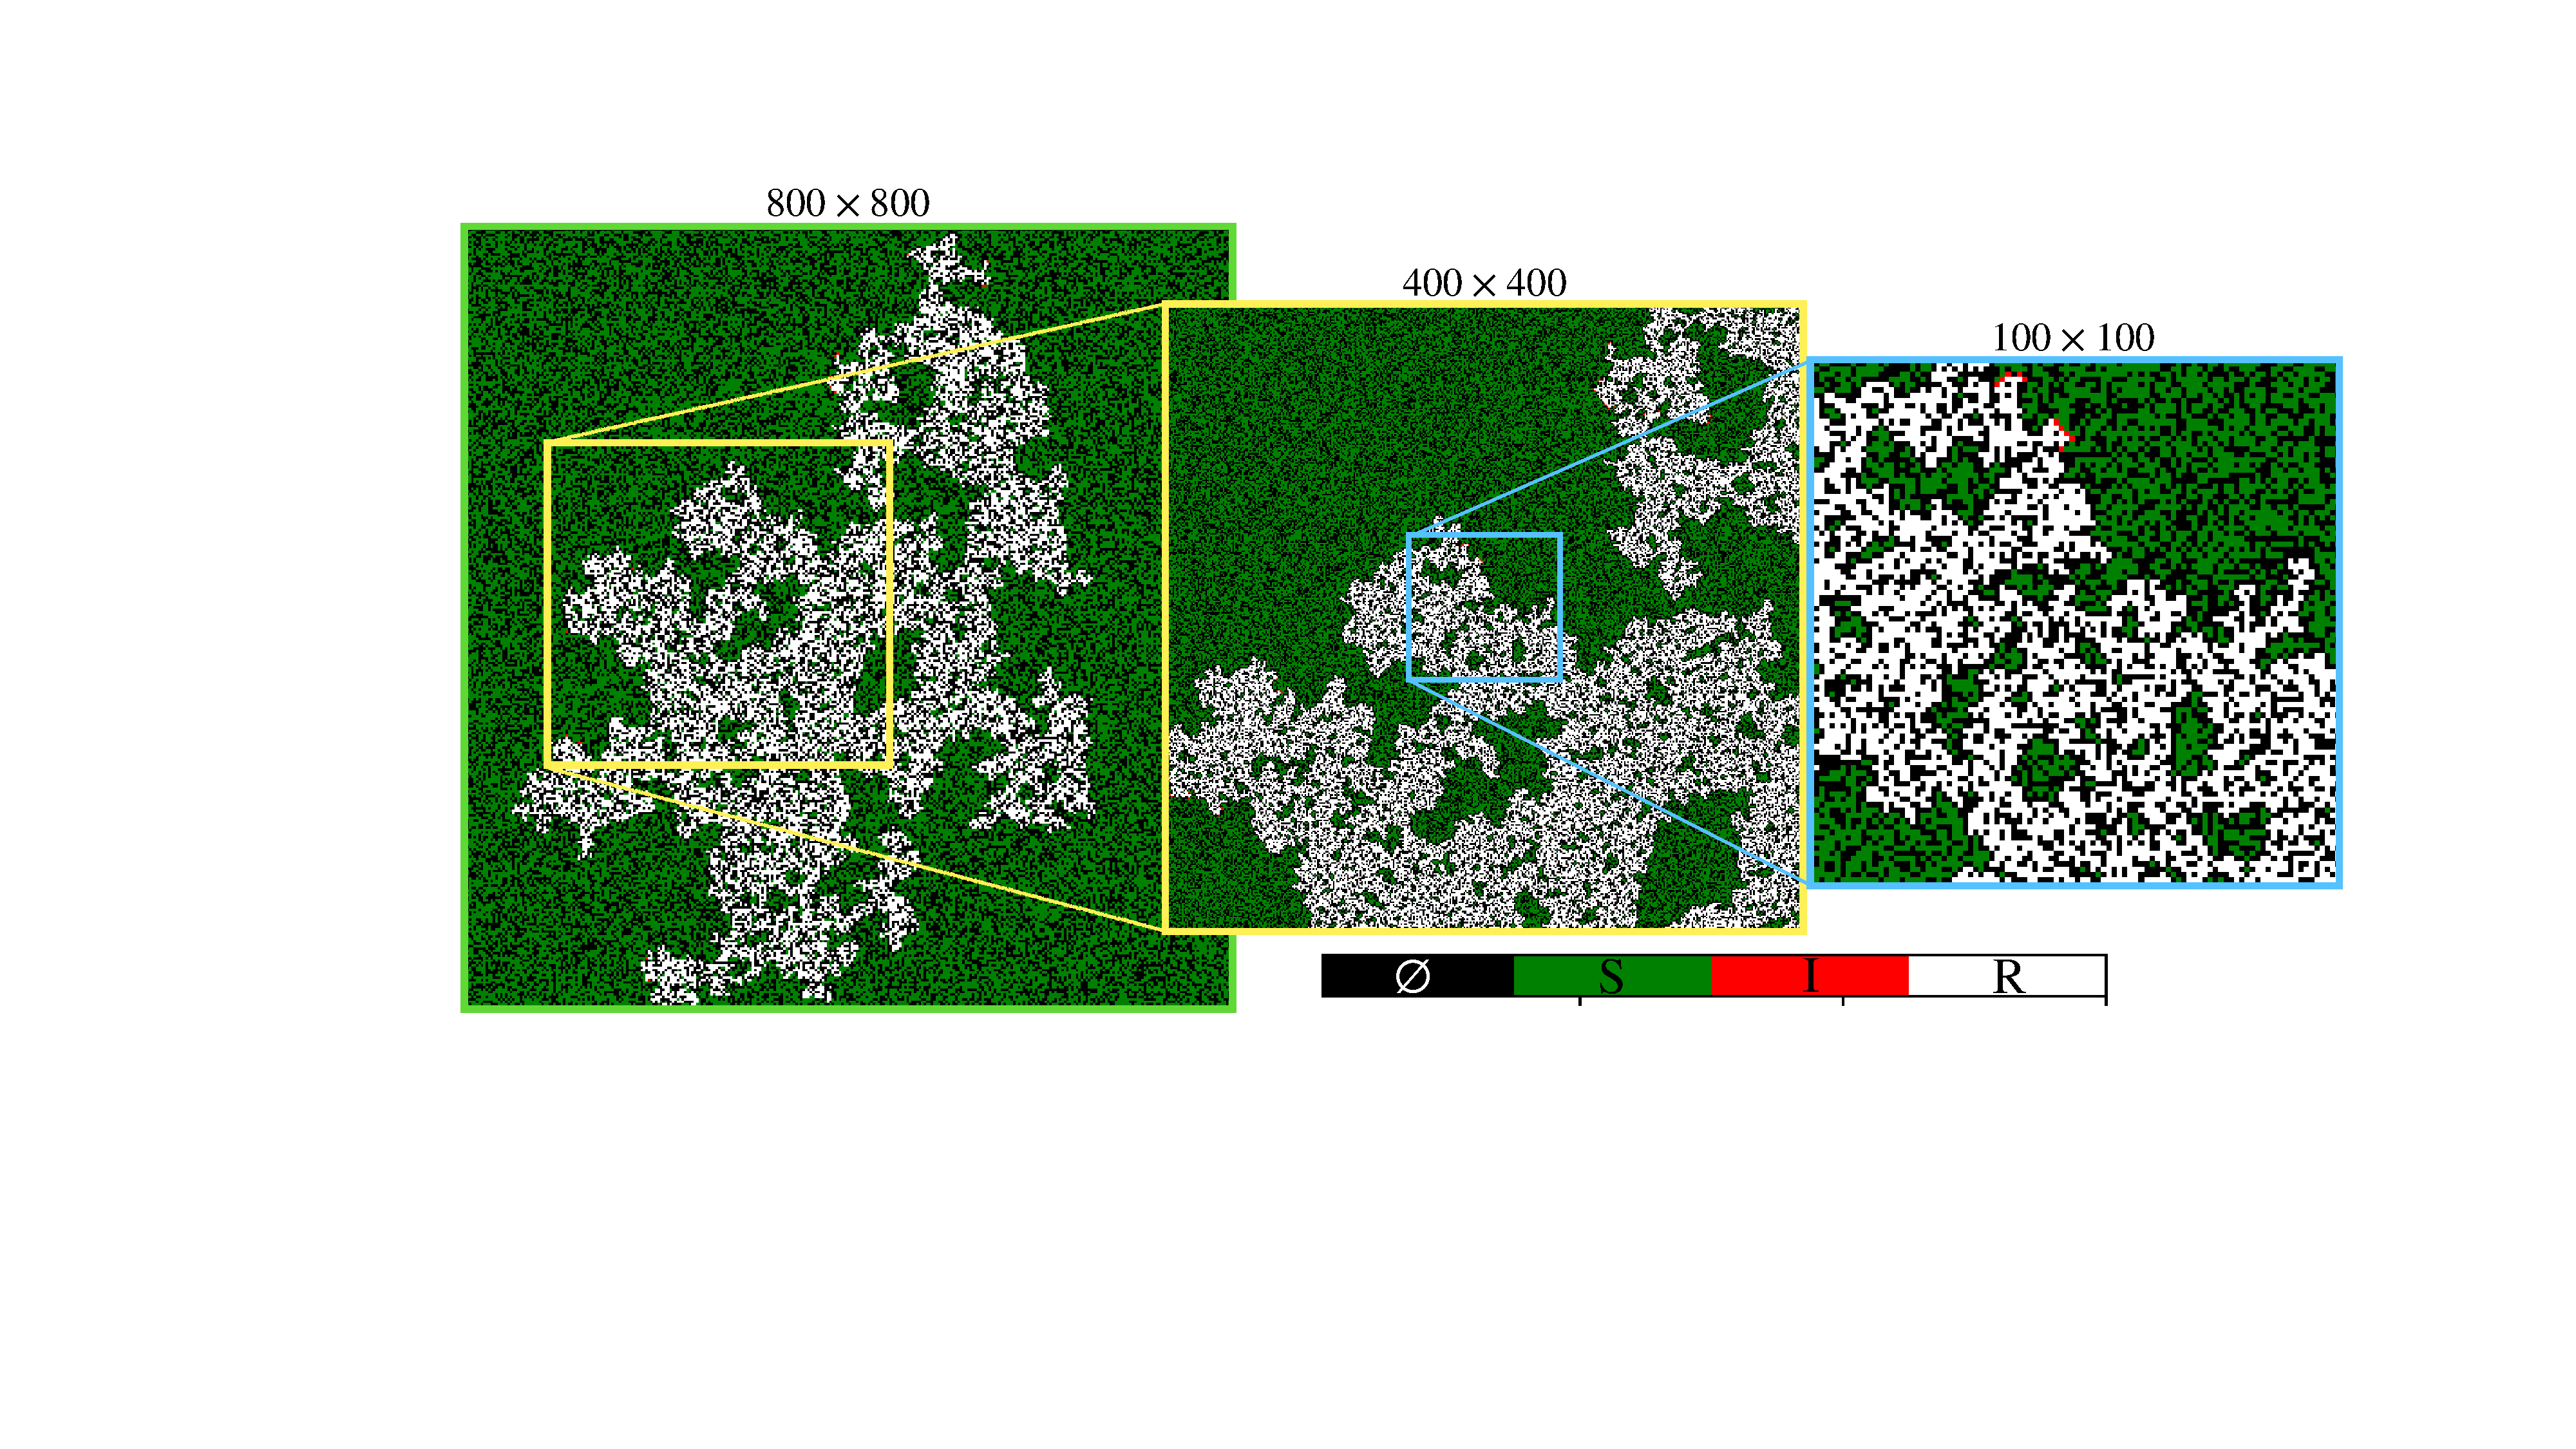
\includegraphics[scale=0.325]{chapter3/figures/figure3.pdf}
    \caption{Scale invariance within the percolation-based $SIR$ model. A cluster spanning the domain at the critical density $\rho_c = 0.592...$ is shown for three different spatial resolutions.}
    \label{fig:ch3-perc-invariance}
\end{figure}

The SLM model used in both this and the proceeding three chapters is based on a square lattice. %
We could have considered many other configurations such as the triangular, honeycomb or Voronoi lattice. %
As such, various quantities within the model would be expected to change as an artifact of the lattice type, %
in particular the numerical value of $\rho_c$, see table \ref{tab:perc} for a table of selected percolation thresholds. %
Therefore, it is worth giving a brief description of criticality and universality within the model. %
This is useful to highlight crucial aspects of percolation and how the model  behaves given alternate lattice configurations. %

At the critical density, the emergence of some interesting phenomena is witnessed. %
Figure \ref{fig:ch3-perc-invariance} shows the spanning cluster of infectious-removed trees (in red and white respectively) at $\rho =\rho_c$. %
The cluster looks remarkably similar at all spatial resolutions and is said to be `self-similar' \cite{Kapitulnik_1983}. %
Within $C_\infty$, one can identify clusters of untouched susceptible trees (in green) of various sizes. %
This suggests a distribution of different cluster sizes that occupy all possible length-scales within the lattice. %
In the literature, clusters within a distribution are described by $n_s$ (the `cluster number'), where $n_s$ is the number of clusters containing $s$ open lattice sites. %

Increasing the lattice size $L$ as $\rho = \rho_c$, the largest cluster present (denoted by $M$) would scale as $M\propto L^{1.9}$ (opposed to $M\propto L^{2}$ for $\rho > \rho_c$). %
This is indicative of the cluster fractal dimension $d_F=1.9$ and is important when considering changes in the size of the lattice. %
If the cluster is normalised by the size of the lattice ($L^2$), the mean density of $M$ would decay with an increase in lattice size, i.e. $L^{1.9}/L^2 = L^{-0.10}$. %
This is a non-intuitive relationship and has implications for finite sized scaling\textemdash see \cite{stauffer2018introduction} for further discussion. %

At $\rho \sim \rho_c$, percolation and scaling theory explain how the system follows a power law of the form $\propto (\rho - \rho_c)^{\alpha}$ where $\alpha$ is a universal critical exponent. %
All systems that possess the same exponent are members of the same `universality class' \cite{PhysRev.180.594, RevModPhys.76.663}. %

Consider the probability that one open site (at the origin) is connected to another open site a distance $r$ away. %
In this scenario, the probability is described by the `correlation function' $g(r)$. %
The behaviour of this function defines a length scale, denoted as the `correlation length' $\xi$ that dictates how the probability of `connectedness' decays with distance $r$. %
For densities close to percolation threshold: %

\begin{equation*}
    \xi \sim |\rho - \rho_c|^{-\nu}
\end{equation*}

This relation can be understood by considering how the connectivity of open sites depend on density and the divergence that occurs at $\rho=\rho_c$. %
For low densities, $\xi$ is clearly small as clusters exist in singlets and triplets etc. %
However, as $\rho$ increases the mean cluster length begins to increase as more sites become open and connect to form larger clusters. %
As the critical density is approached from the direction $\rho \rightarrow \rho_c^{-}$, the spanning cluster is formed and $\xi$ diverges from large finite values towards infinity, $\xi \rightarrow \infty$. %
If one neglects the divergent spanning cluster, a similar picture is painted for densities just above criticality $\rho > \rho_c$. %
The correlation length $\xi$ decays rapidly as $|\rho - \rho_c|$ increases. %
This time however,  mid-large sized clusters get absorbed by $C_\infty$ as the density increases. %
This leaves only small clusters untouched and $\xi \rightarrow 0 $ as $\rho \rightarrow 1$ \cite[see][for a detailed break-down of power laws and correlation length.]{STAUFFER19791}. %

Importantly, the critical exponent $\nu$ is universal for all lattice types and only depends on the dimension of the lattice used. In general, there are different critical exponents for various quantities however, as shown by \cite{stauffer2018introduction, STAUFFER19791}, all follow similar power laws. 

If the system crosses the percolation threshold, it can be likened to a phase-transition. %
Subsequently, the terms `phase-transition' and `percolation' will be used interchangeably throughout this work. %
Broadly speaking, the critical phenomena found in percolation theory, thermodynamics and magnetism have close ties and are described by similar power laws underpinned by scaling theory \cite{Essam_1980}. %

\section{Introducing infectivity\textemdash a two parameter model}
\label{ch3:two-param-model}

We have established a percolation-based model of tree disease described by a one-dimensional parameter-space over tree density $\rho$. %
We now extend the parameter-space to include an `infectivity' parameter, denoted by $\beta$. %
Previously, an assumption was made about pathogen-transmission, namely: %
infected trees will transmit the infection to susceptible nearest neighbours with perfect fidelity, %
that is, a probability of $1$. In reality, pathogens display a range of different infectivities depending on the virulence of the strain (or susceptibility of the host). %
This is captured by infectivity $\beta$. 

The probability of a susceptible tree becoming infected during one time-step is given by: %
$Pr(S \rightarrow I) = \beta$ (see appendix \ref{a:propagation} for a description of how this is implemented computationally). %
The infectivity parameter describes a transmission `rate' (i.e. per time-step) and is closely linked to the infectious life-time $T$ of the tree. %
The probability a susceptible tree will remains such  when neighboured an infected tree is given by:

\begin{equation}
\label{eq:pr_s_s}
    Pr(S \rightarrow S) = \rho(1 -\beta)^T
\end{equation}
As the infectious life-time gets larger the probability of remaining susceptible decreases. %
A susceptible tree will now become infected and survive for $t=T$ time-steps before transitioning into $R$. %
Equation (\ref{eq:pr_s_s}) sets the basis for a mean-field theory (see appendix \ref{a:slm-mean-field-theory}) and connects $\beta$ and $T$. %
This two-parameter model used by \cite{OROZCOFUENTES201912} will be refereed to as the simple lattice model (SLM). 

Figure \ref{fig:slm} shows the SLM spreading through three time-steps with fixed values of $T=10$, $\rho=0.70$ with variations in $\beta$. %
Different stages through the infectious period are shown in the colour bar from yellow-red. %
Higher values of $\beta$ yield a faster spreading velocity. %
Figure \ref{fig:slm} alludes to $\beta$ altering the percolation threshold as simulations for a low infectivity of $\beta=0.25$ reveal not only a slower spreading velocity but a more fractal-like spreading pattern. %

\begin{figure}
    \centering
    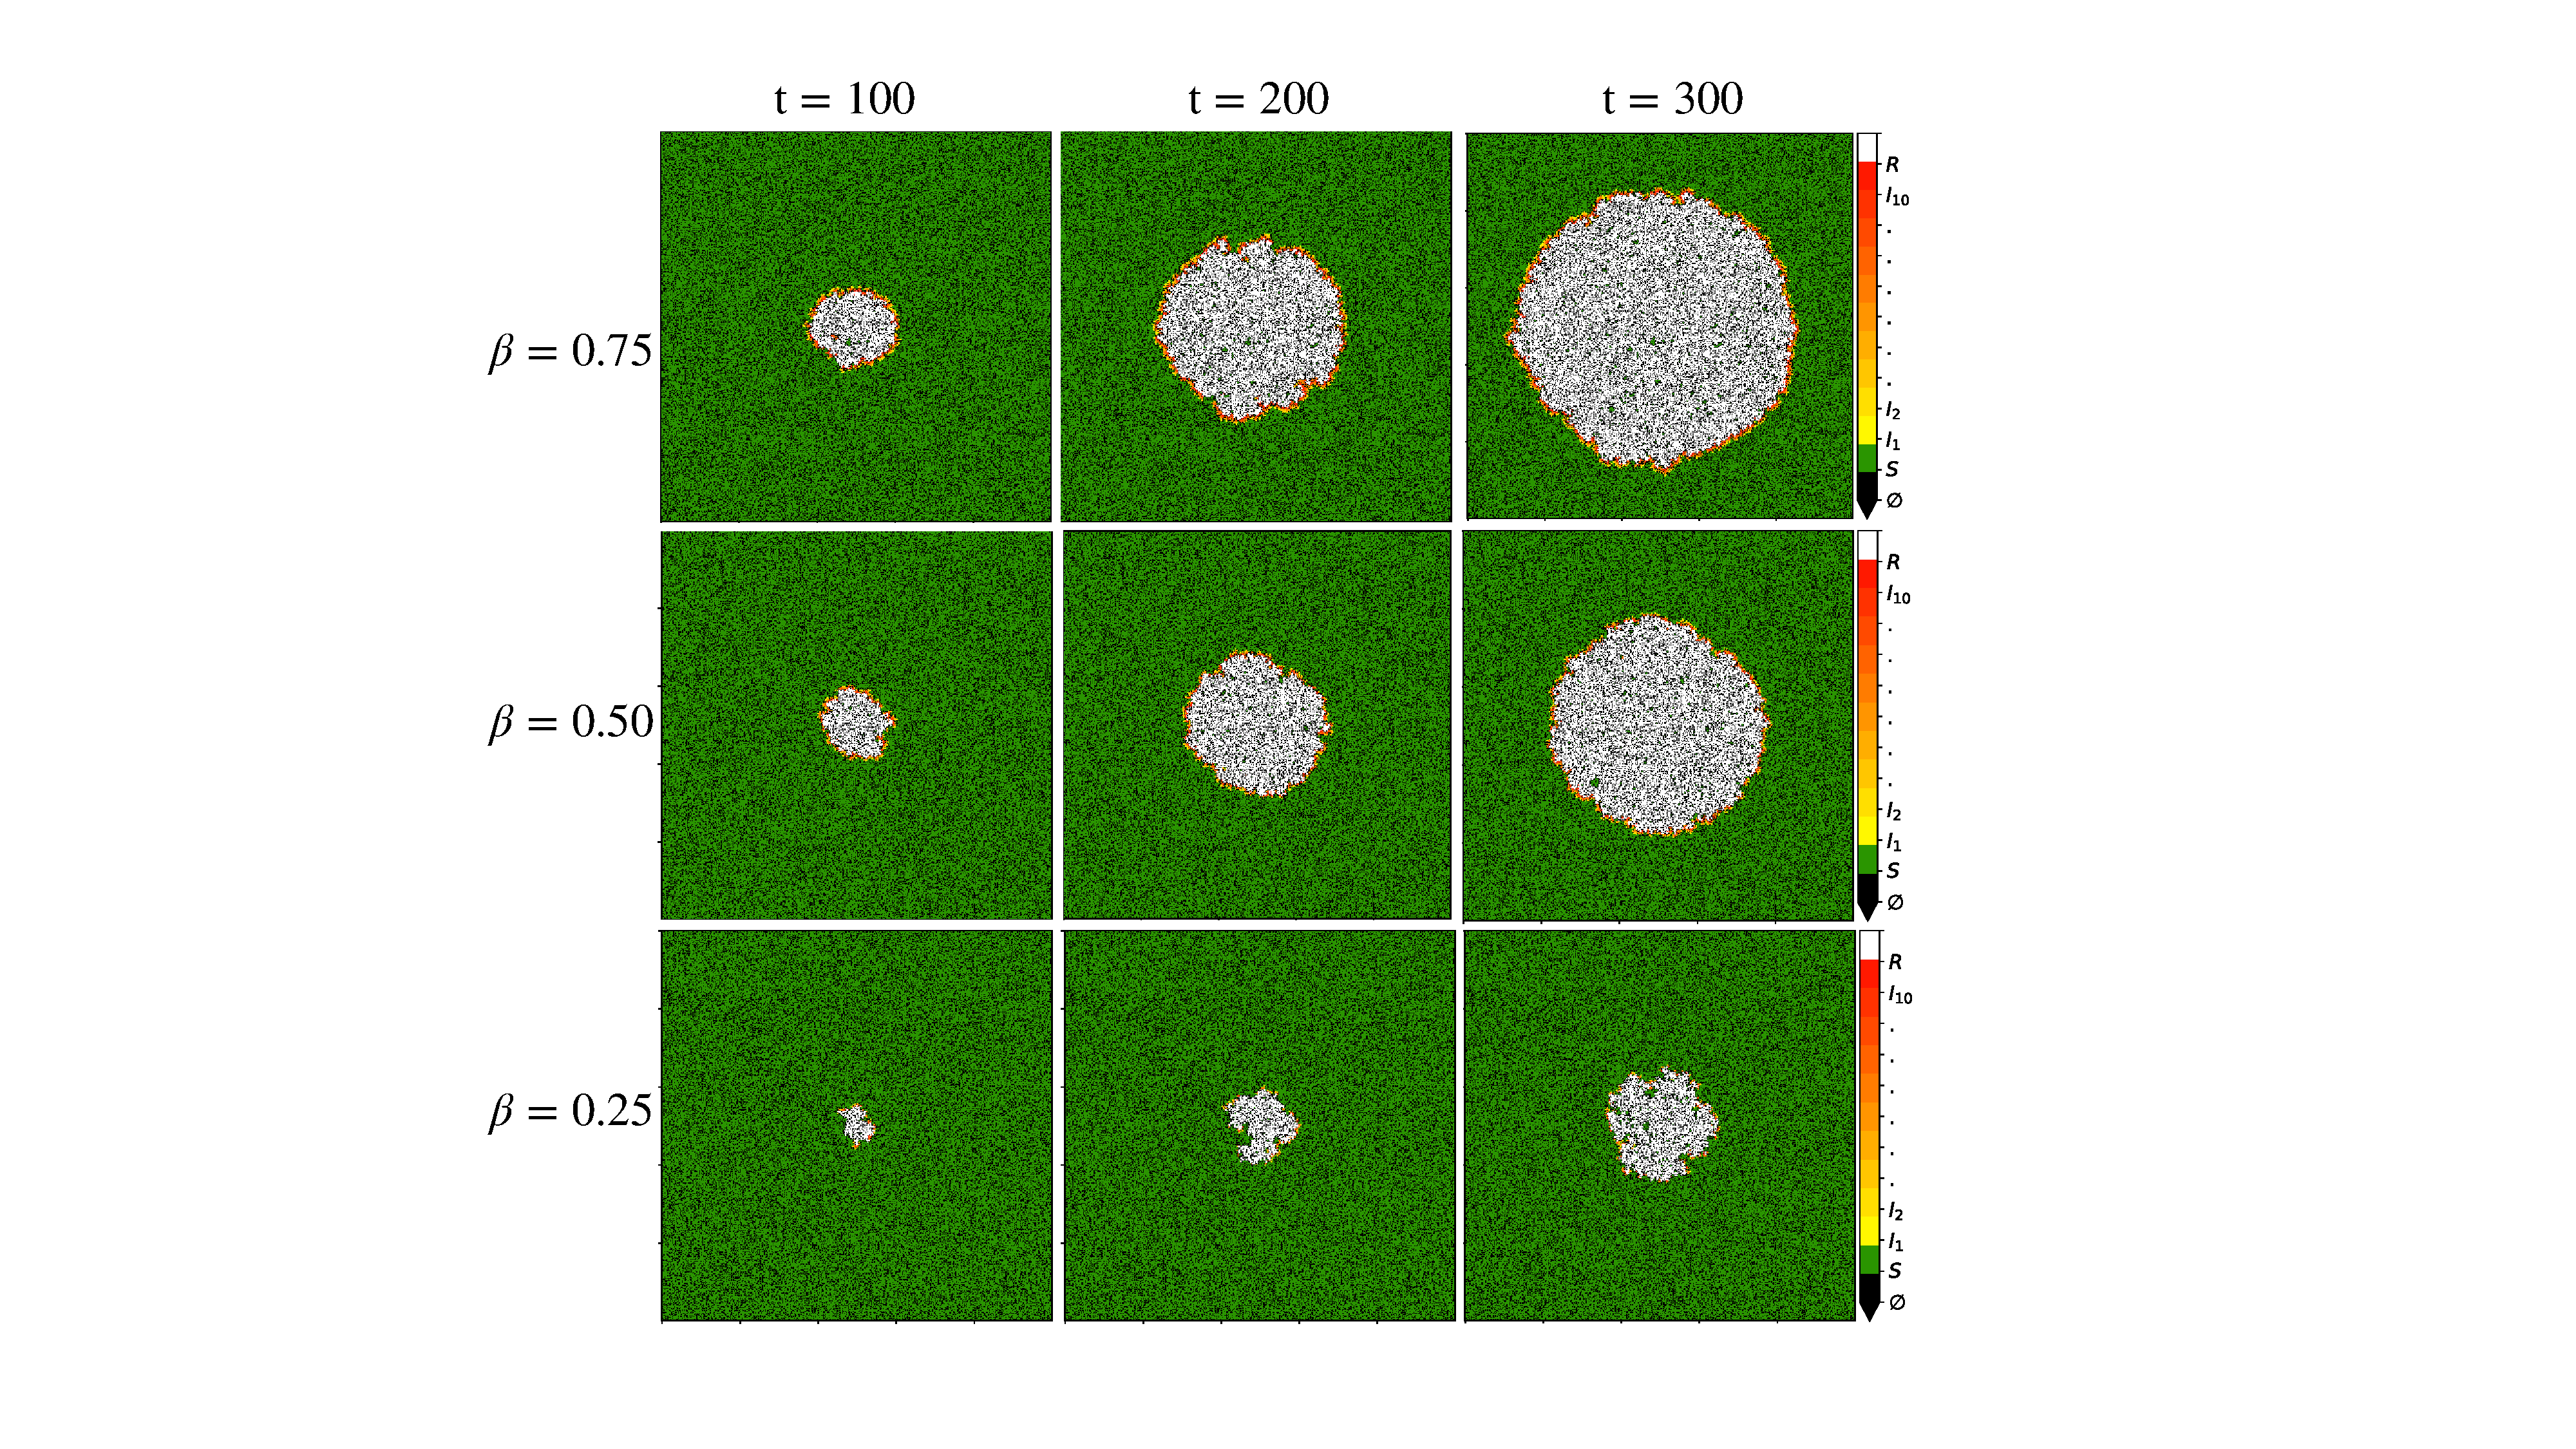
\includegraphics[scale=0.4]{chapter3/figures/figure5.pdf}
    \caption{Introducing an infectivity parameter $\beta$. The SLM is shown running on a domain of size $500\times500$ for fixed $T=10$ and density $\rho=0.70$. Simulation reveal that $\beta$ has an impact on the wave-front speed and changes the percolation threshold.}
    \label{fig:slm}
\end{figure}

\begin{figure}
    \centering
    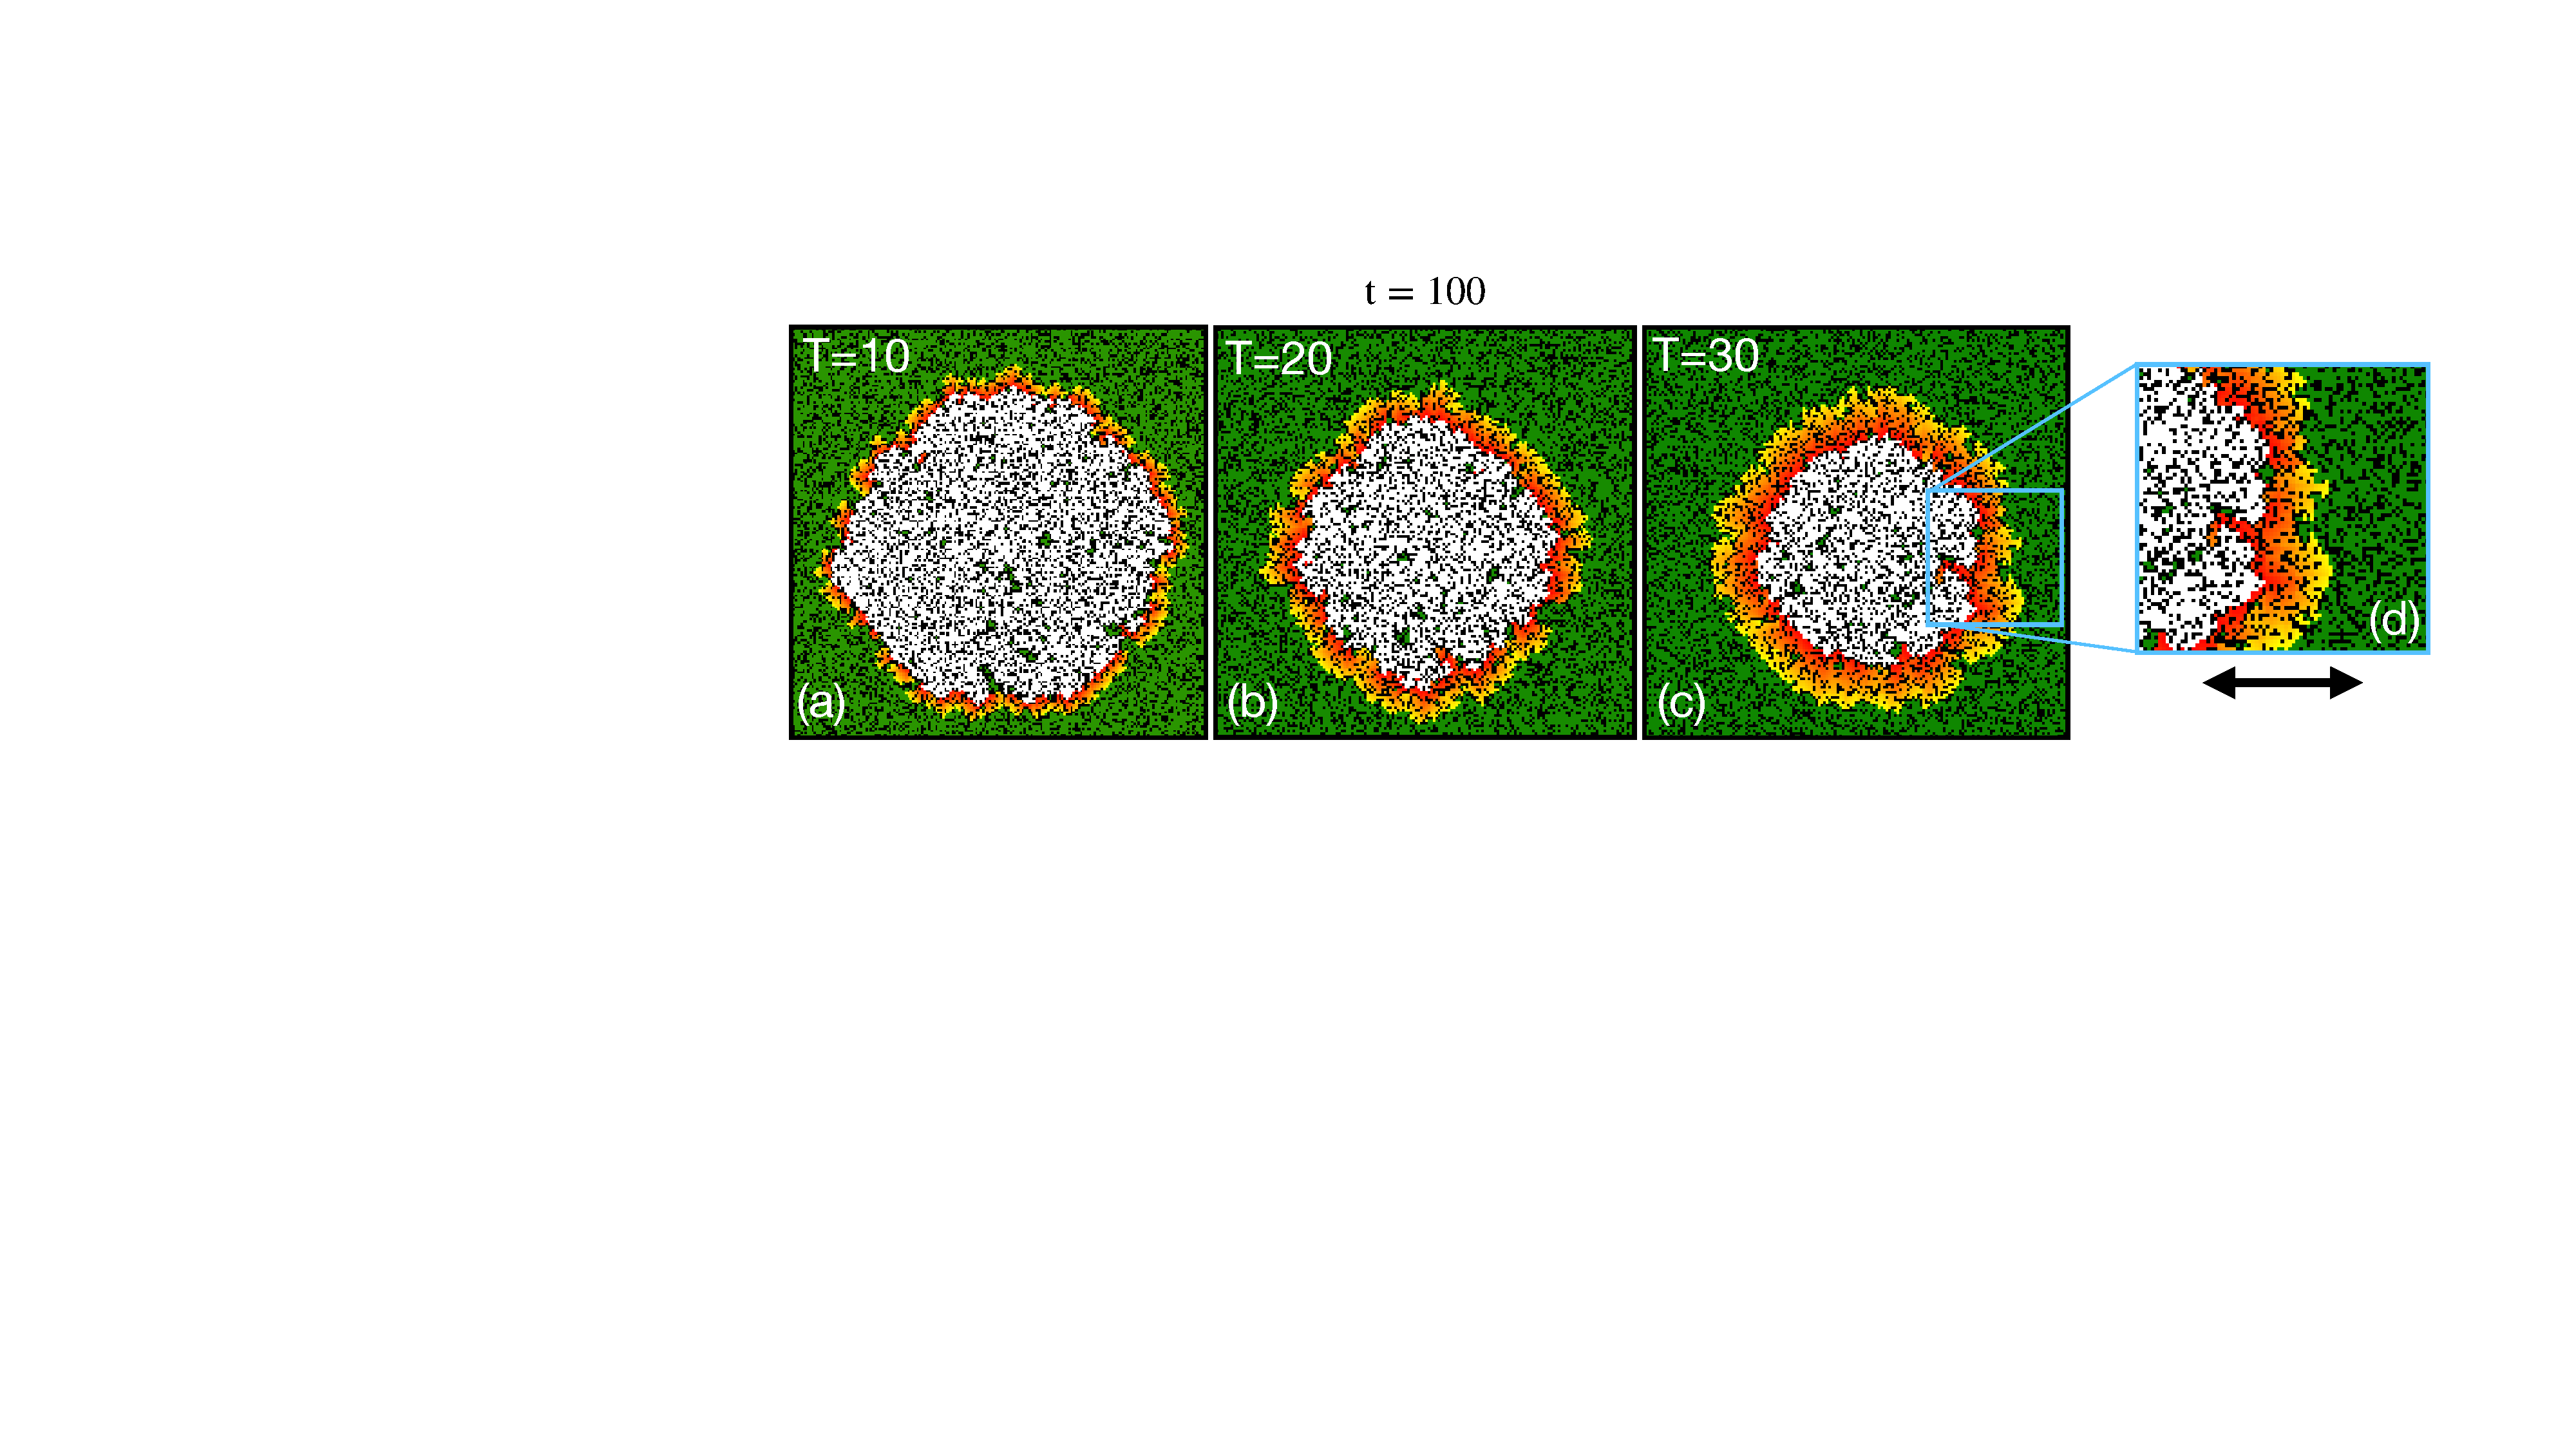
\includegraphics[scale=0.35]{chapter3/figures/figure5_.pdf}
    \caption{Simulations through a single time-slice for fixed density and infectivity reveal that increases in the infectious life-time $T$ has little impact on the speed of the wave-front interface (the boundary between $S$ and $I$). However, increasing $T$ leads to a lag in the posterior of the wave-front (the boundary between $R$ and $I$).}
    \label{fig:slm-wave-front}
\end{figure}

Figure \ref{fig:slm-wave-front} shows how variations in the infection life-time can change the wave-front properties. %
The value of $\beta$ predominantly controls the speed of the  wave-front whereas $T$ controls the lag-time on the removal front. %
Increasing  $T$ yields an  increase in the wave-front thickness. %
This is valid for $\rho > \rho_c$ however, for $\rho \sim \rho_c$ the relationship between $T$ and spreading velocity is less obvious. %
Close to percolation threshold, variations in $T$ have more importance and could lower or raise transmission rates below or above percolation thresholds, respectively. %

For the purposes of building a simple lattice model upon which to elaborate, the spreading velocity is an important behaviour to understand. %
Given that $\beta$ is more relevant for the wave-front speeds, arbitrarily fixing the infection life-time to $T=10$ will not detract from our understanding of the spreading behaviour. %
This allows us to explore a simplified two parameter ($\rho, \beta$) model. %
The definition of critical threshold can now be generalised from Eq (\ref{eq:critical_threshold_1d}) to include the parameter $\beta$: %

\begin{equation}
\label{eq:critical_threshold_1d}
    \rho _{c}=sup \lbrace \rho, \beta : \theta (\rho, \beta ) = 0 \rbrace
\end{equation}

\subsection{Phase-transition and ensemble averaging technique}

The percolation threshold occurs between a narrow range of parameters and no information regarding the rate of propagation is captured. %
In order to capture spreading rates, a metric comprising the spreading velocity is introduced: %
\begin{equation}
\label{eq:vel_eff_r}
    v_{radial(t)}=\sqrt{N_I(t+1)-N_I(t)}
\end{equation} 
Where, $N_I$ is the number of infected trees in the domain at time-step $t$. %
The difference in $N_I$ between time-steps gives an `effective' radial velocity. %
That is, the number of spatial units progressed by the pathogen averaged over all angles per unit time. %
Strictly speaking, Eq (\ref{eq:vel_eff_r}) is valid only for $\rho > \rho_c$, %
at the percolation threshold the wave-front assumes a fractal dimension and averaging over two dimensions becomes unreasonable\textemdash
see \cite{OROZCOFUENTES201912} for information on the fractal dimension and wave-front. %

The time-series, $v_{radial}(t)$ is shown in Figure \ref{fig:vel_eff_rad_metric}(a) for three high-low combinations $(\rho, \beta)$. %
Variance in the time-series is greatest through the first $\sim 200$ time-steps, %
this is a consequence of the initial conditions and suggests the system has yet to reached a steady state \textemdash %
the system is said to be in a `transient' state. %
A state of initial instability is regularly seen in the study dynamical systems. %

\begin{figure}
    \centering
    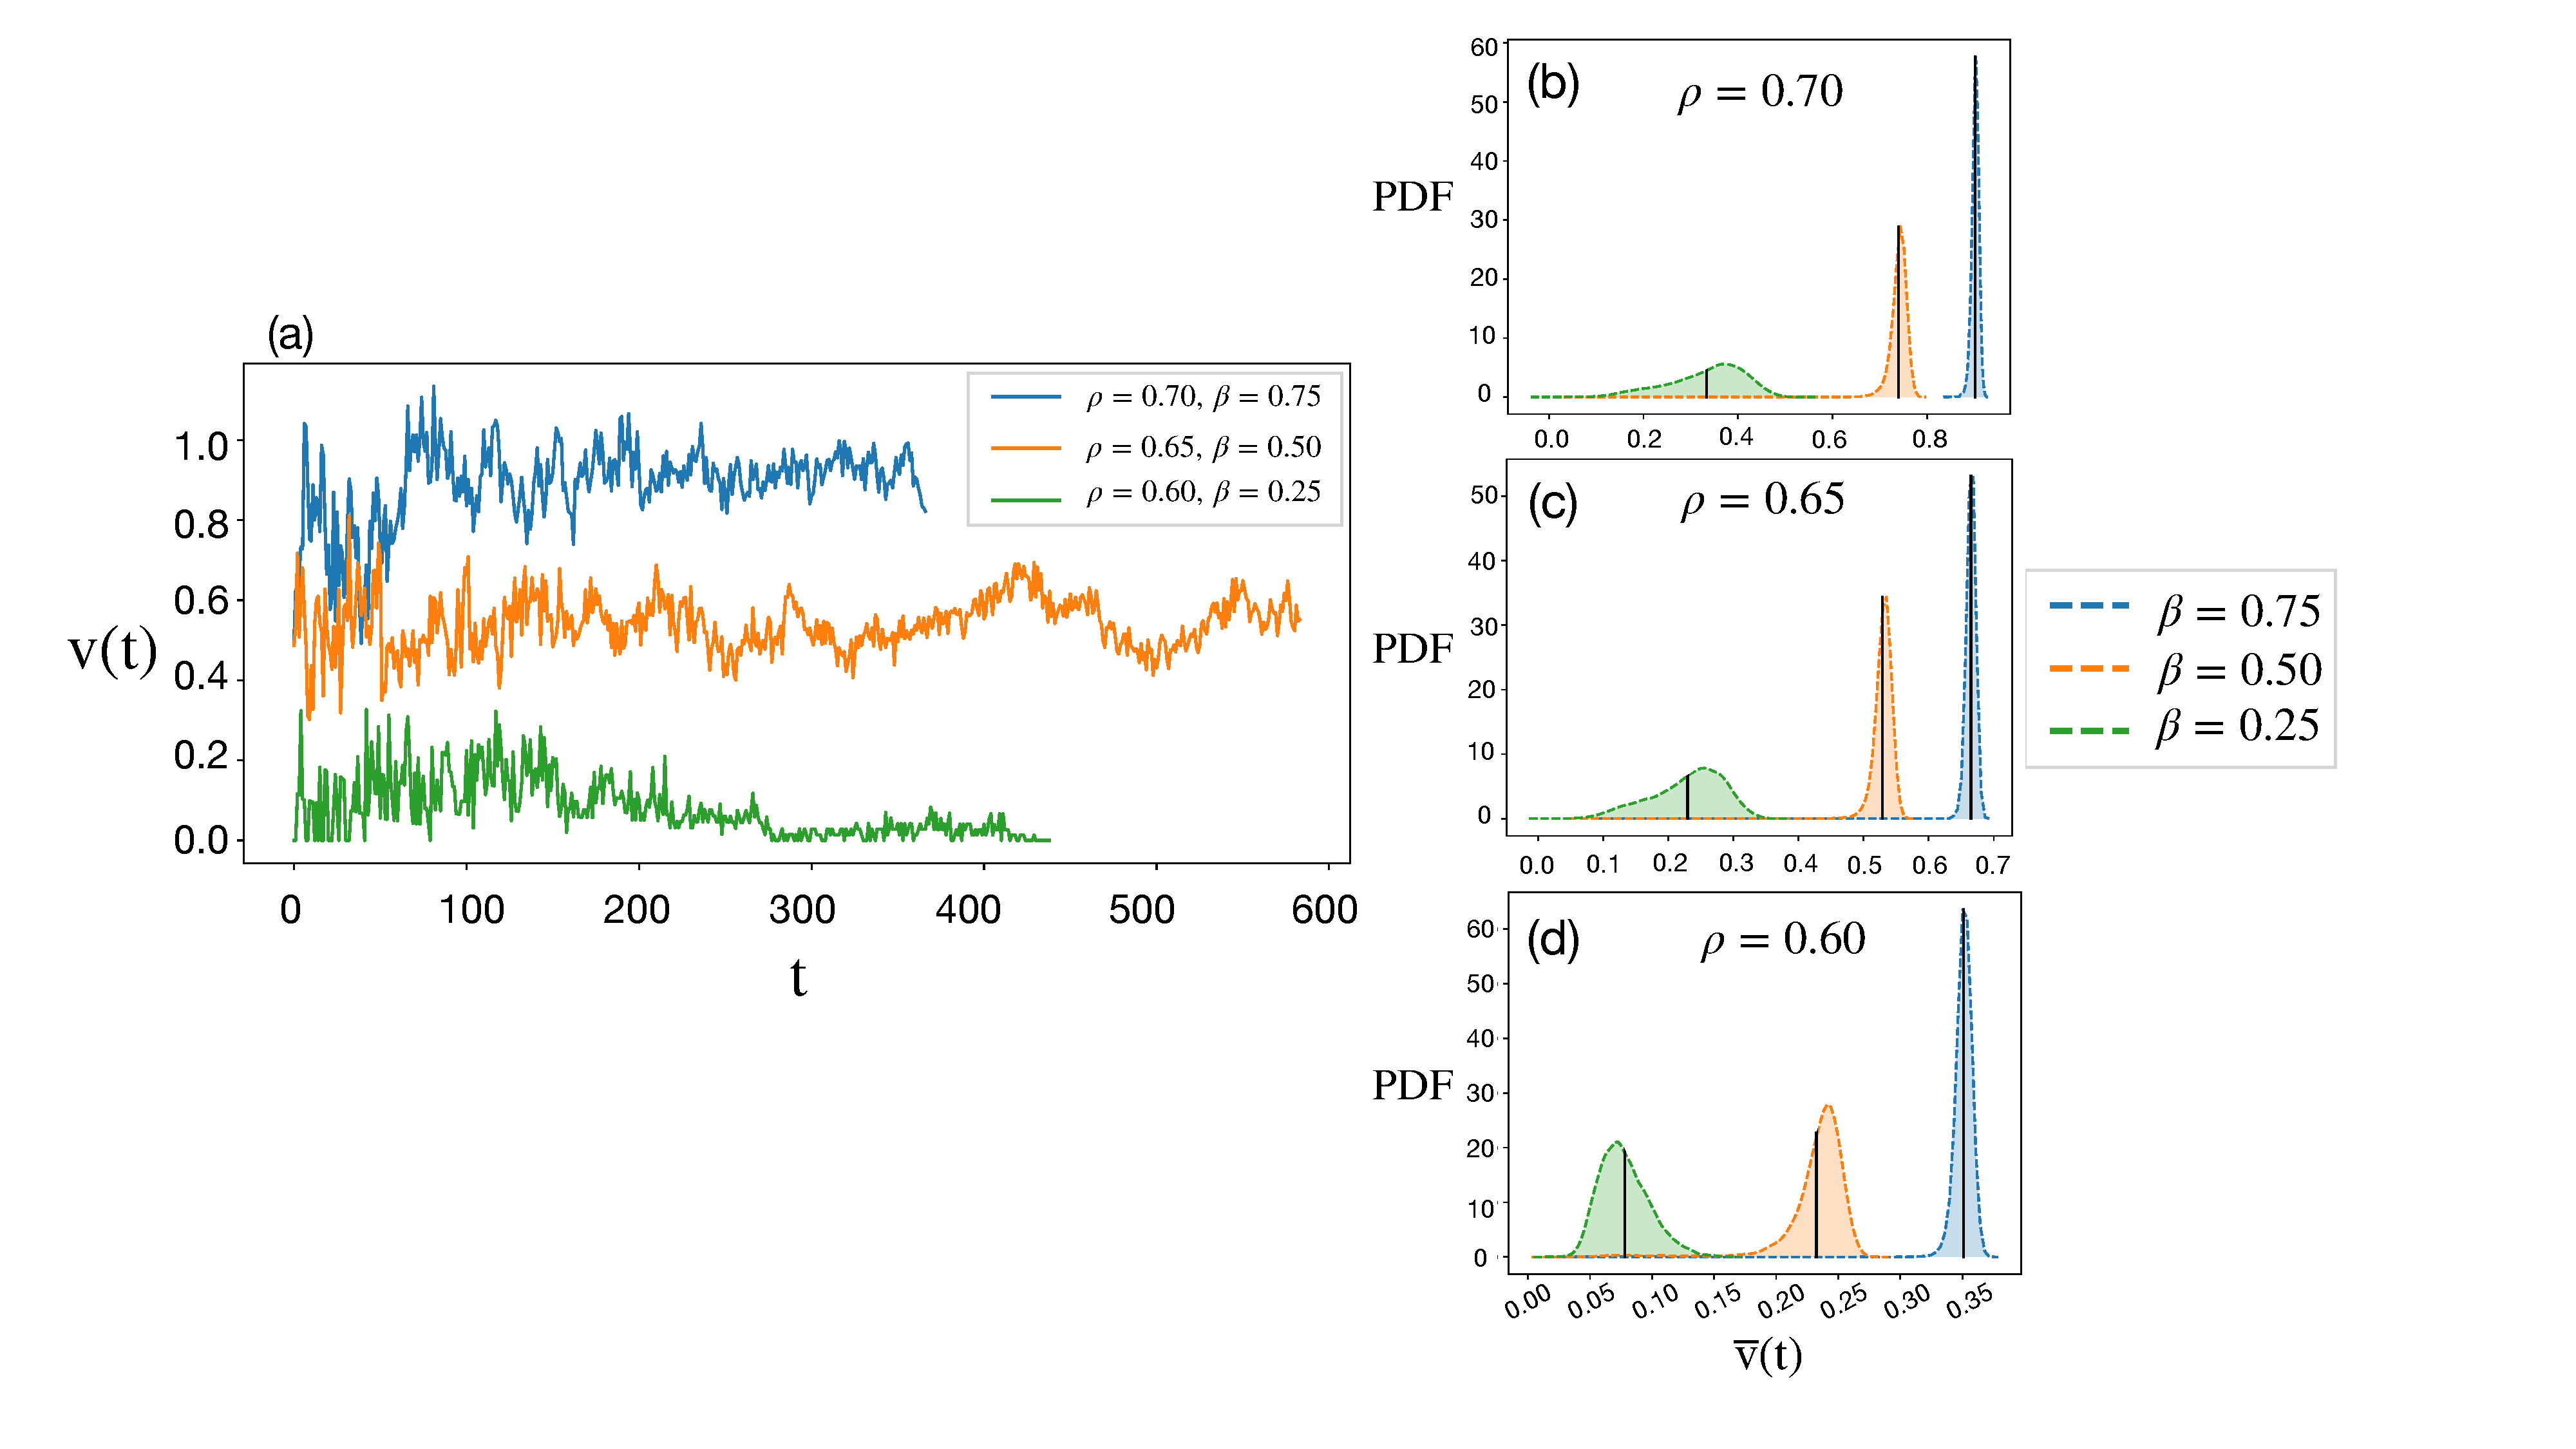
\includegraphics[scale=0.26]{chapter3/figures/figure7.pdf}
    \caption{(a) The velocity metric time-series $v_{radial}(t)$ is shown for three typical simulations, higher values of $\rho$ and $\beta$ give higher mean values of propagation speed. (b-d) The probability density function of mean spreading velocity $\big\langle \overline{v}_{radial}(t) \big\rangle$ for variations in $\rho$ and $\beta$.}
    \label{fig:vel_eff_rad_metric}
\end{figure}

\begin{figure}
    \centering
    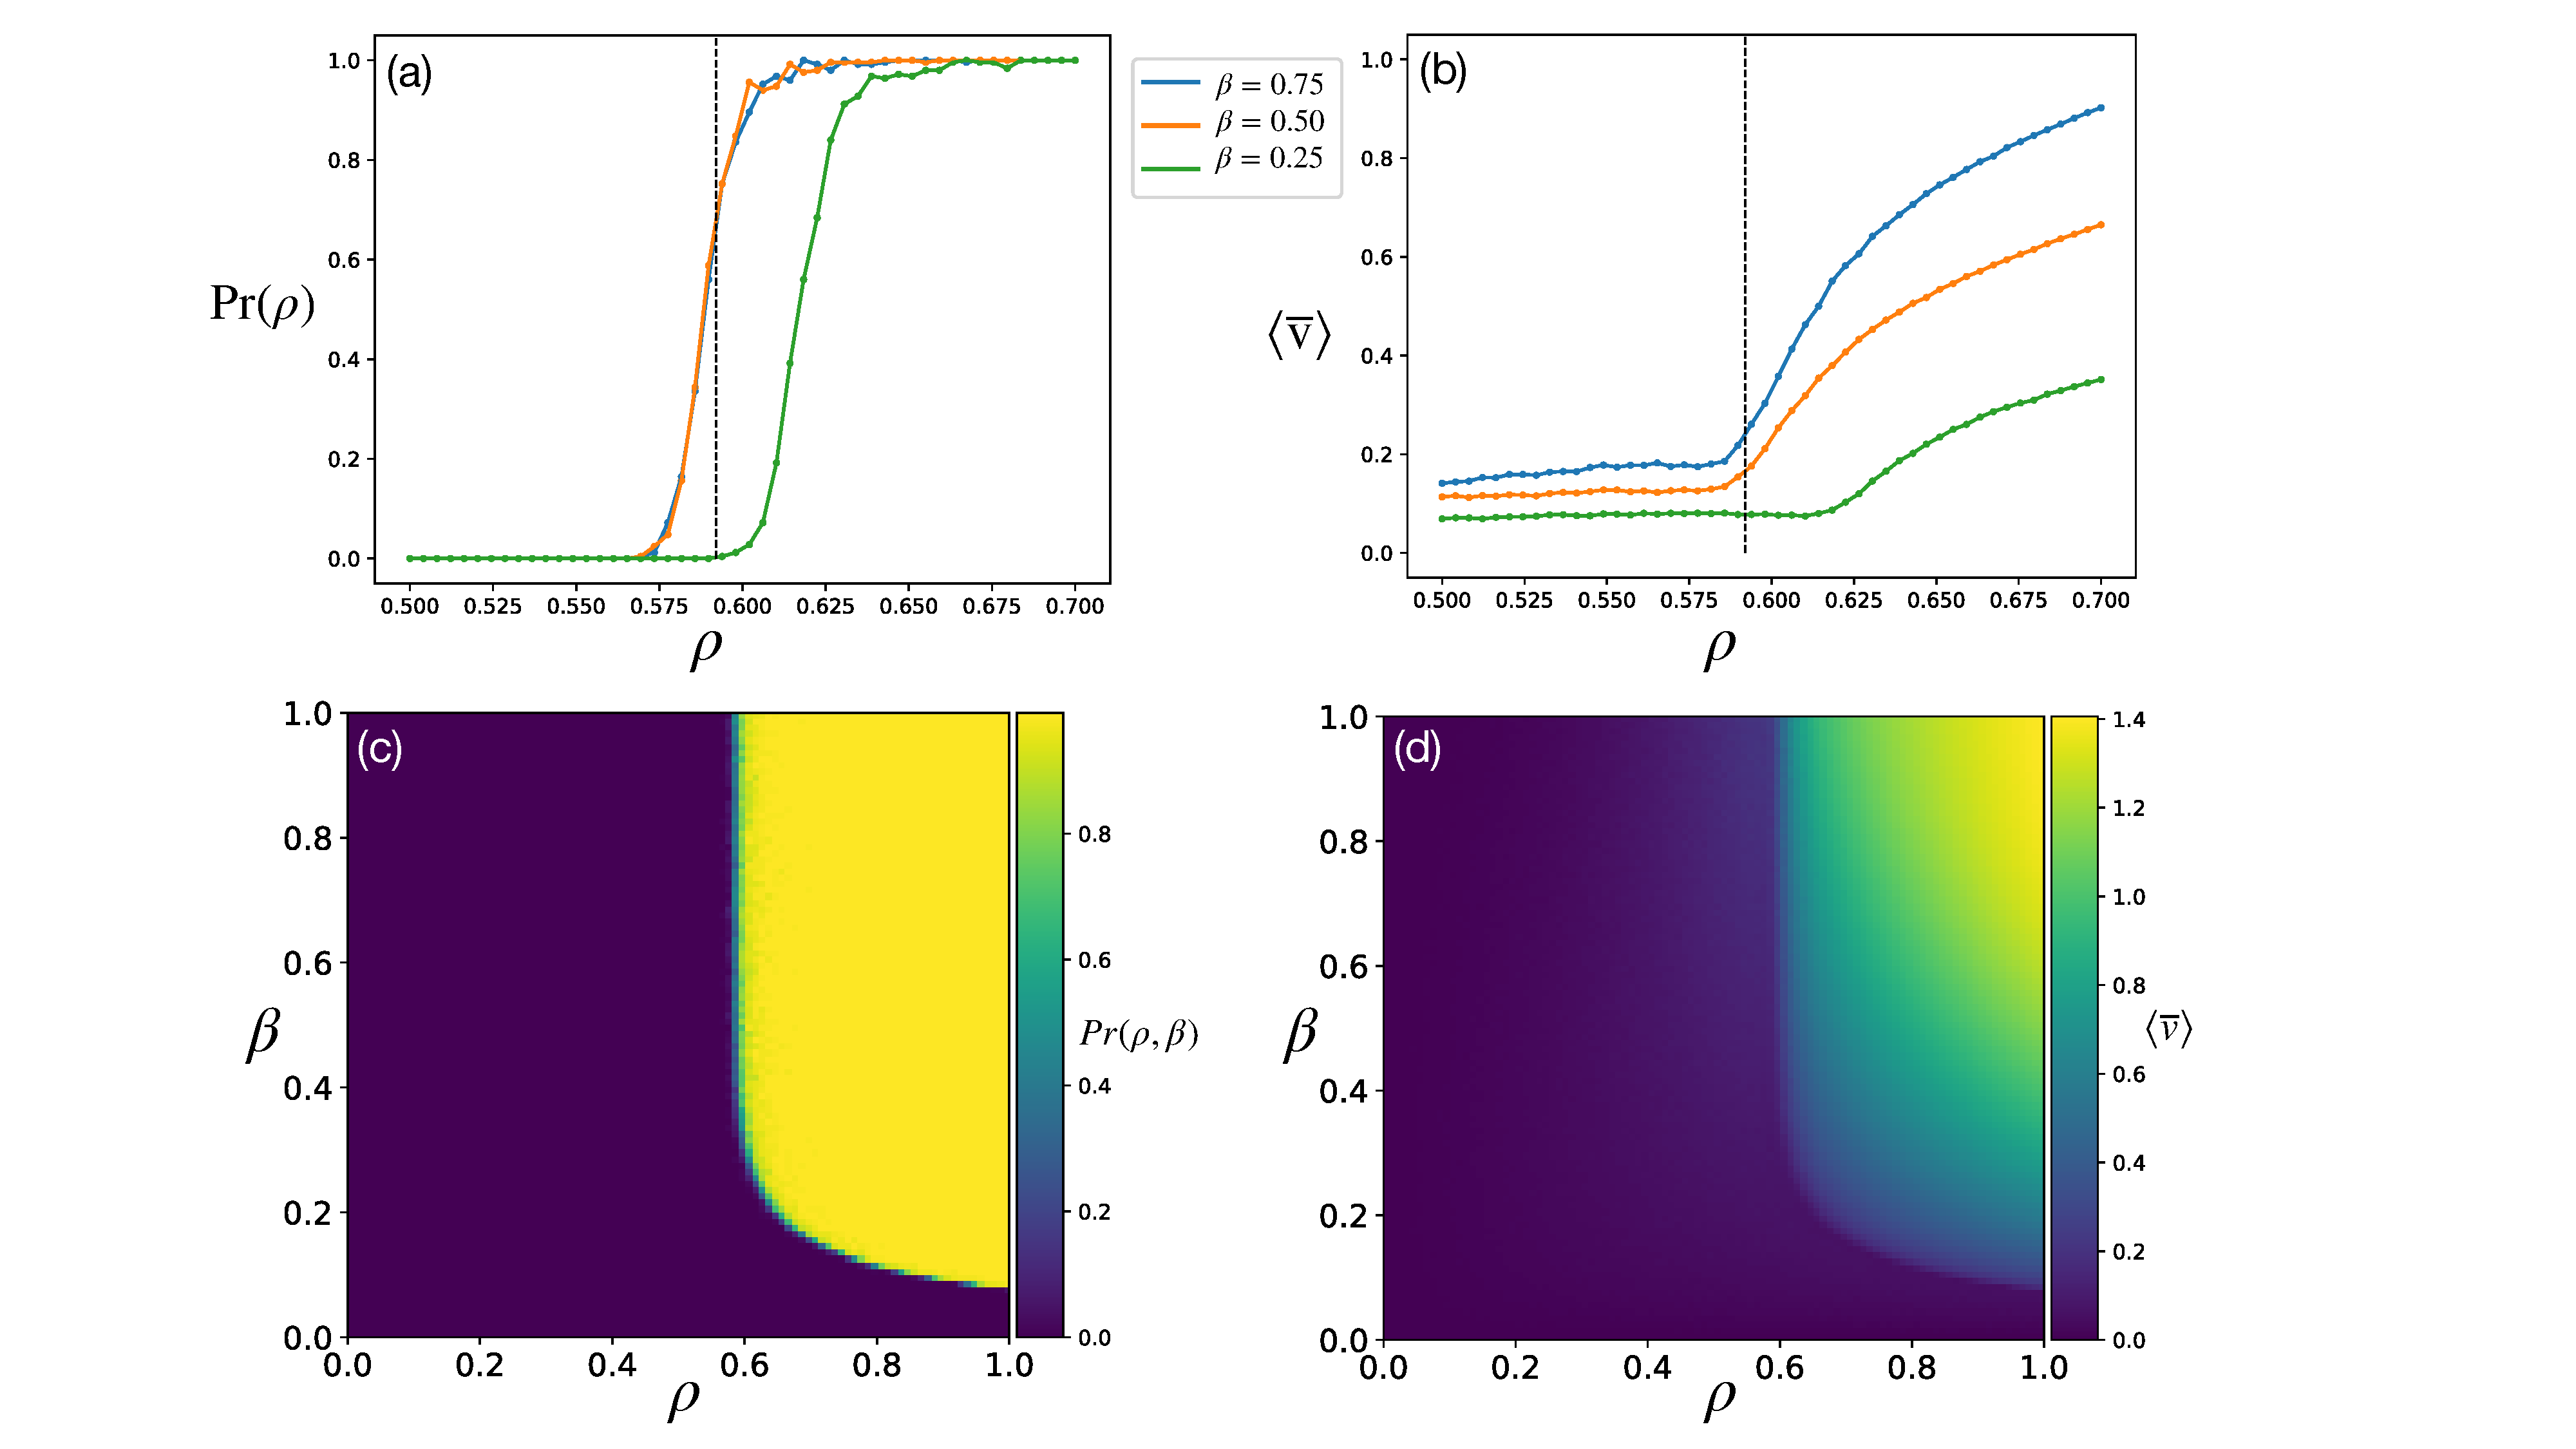
\includegraphics[scale=0.325]{chapter3/figures/figure8_.pdf}
    \caption{A parameter sweep of $\rho$ and $\beta$ over the $500\times500$ domain. (a-b) The percolation probability is shown alongside the radial velocity over a one-dimensional parameter-space of $\rho$. For the lower-valued infectivity of $\beta=0.25$, the density threshold is slightly higher than classical percolation  $\rho_c=0.592$, indicated by the vertical dashed line. A gradual increase occurs when using the radial velocity whereas percolation shows an abrupt transition. (c-d) A two-dimensional parameter sweep  paints a similar picture.}
    \label{fig:slm_pspace}
\end{figure}

In Figure \ref{fig:vel_eff_rad_metric}(a), a simulation average $\overline{v}_{radial}(t)$, can be  determined and plotted as a horizontal line. %
Repeating this measurement multiple times, over an `ensemble', gives a probability distribution. %
Example  probability density functions are shown in Figures \ref{fig:vel_eff_rad_metric}(b-d) for different parameters.%

Statistical measures over the ensemble have interesting applications and can be used to detect an EWS (discussed later). %
For now, the important statistic is merely the average shown by the vertical black %
lines\footnote{Any simulation that became extinct before the initial transient period, %
of $t_{tr}\approx 200$ time-steps, was excluded from calculations of the ensemble mean.}. %
The ensemble average $\big\langle \overline{v}_{radial}(t) \big\rangle$ is used to determine the spreading velocity at position $(\rho, \beta)$ in parameter space. %
For brevity, the ensemble average will be denoted by $\big\langle\overline{v}\big\rangle$, unless otherwise stated. %

Figure \ref{fig:slm_pspace} shows the model behaviour using both the percolation and velocity metric. %
In Figure \ref{fig:slm_pspace}(a), a one-dimensional line through the parameter-space of $\rho$ reveals the probability of percolation for three different infectivity parameters\textemdash the accepted percolation threshold for a two-dimensional square lattice is shown by the vertical dashed line. %
For $\beta \in [0.50, 0.75]$, the probability of percolation is identical to that shown in Figure \ref{fig:ch3-perc-pr}, although a lower value of $\beta = 0.25$ shows a decreased percolation threshold. %

In Figure \ref{fig:slm_pspace}(b), the ensemble averaged time-series, denoted by $\big\langle \overline{v} \big\rangle$, gives a similar yet different trend. %
When the density crosses the percolation threshold, marked by the vertical dashed line, a sharp increase in the speed of propagation can be seen. Additionally, higher values of $\beta$ yield a higher effective radial-velocity. %
Crucially, when this metric is used more information is captured about the dynamical behaviour of pathogen. %

Ensemble results over a two-dimensional parameter-space of $\rho$ and $\beta$ are shown in Figures \ref{fig:slm_pspace}(c-d), %
for percolation and radial-velocity respectively. %

In Figure \ref{fig:slm_pspace}(c), the probability of percolation depicts an abrupt transition between two stable regimes of extinction and epidemic. %
Regimes are separated by a narrow range of critical parameters $\rho_c$ and $\beta_c$. Figure \ref{fig:slm_pspace}(d) shows the ensemble averaged velocity metric and again, %
reveals a similar picture. %
This time however, a smoother transition between states is demonstrated. %

In Figure \ref{fig:slm_pspace}(c), the percolation threshold of $\rho_c \sim 0.60$ does not depend on infectiviy beyond the value $\beta>0.30$. %
Between $0.15 <\beta<0.30$, a higher value of $\rho$ is needed for percolation to occur. %
Below $\beta=0.30$ the probability of percolation is zero and a threshold in infectivity $\beta_c \sim 0.15$ is demonstrated. %
Given an incrase in the infectious life-time $T$, $\beta_c$ would shift towards a lower value %
 i.e. the critical infectivity would decrease due to \textit{more} infectious time-steps %
 increasing the probability of transmission, thus lowering the threshold. %
 Here, the parameter-sweeps are analogous to a phase-diagram. %

\section{Early warning signals\textemdash detection and method}

Applications of early warning signals were investigated by \cite{OROZCOFUENTES201912} for forest management and ecosystems-services
\textemdash for a review on early 
warning signals and critical-slowing down in landscape ecology, see Section \ref{section:ews}. 
The work of \cite{OROZCOFUENTES201912} concentrated on a one dimensional parameter space of %
tree density $\rho$ over a square lattice. %
Statistically significant changes (or signals) in the moment-generating functions, %
that being variance, skew and auto-correlation, were calculated from the ensemble distributions of Figures \ref{fig:vel_eff_rad_metric}(b-d). %
Observations of these statistical measures can be used to preempt phase-transitions into the epidemic regime. %
This is useful information that could aid forest and plantation managers to maintain tree health. %

Here, we offer a small extension to some of the concepts presented by \cite{OROZCOFUENTES201912}. %
In particular, a new domain and metric is used that allows for clearer, more realistic early warning signals.  %
Additionally, analysis is generalised to two-dimensions in the parameter-space of $\rho$ and $\beta$. %
After introducing these alternative concepts, we discuss some of the problems and complexities encountered with ensemble-averaging. %

\subsection{Alternative early warning detection}

In order to detect an early warning signal, an assessment of  the temporal variability of the system is needed. %
The findings of \cite{OROZCOFUENTES201912} were gathered by first producing a distribution of \textit{mean} time-series velocities $\overline{v}(t)$, %
analogous to Figures \ref{fig:vel_eff_rad_metric}(b-d). %
The variance, skewness and autocorrelation were then calculated over these distributions. %
In this scheme, an early warning signal is detected from the \textit{variance of the mean} velocity i.e. $var\big\langle \overline{v}(t) \big\rangle $. %

% ALREADY REMARKED OUT
% This is permissible in an abstract setting, however measuring an ensemble of mean velocity values is not possible in practice as there is no way to measure an ensemble of $\langle\overline{v}(t)\rangle$.
% although in theory one could extend this analysis to a more sophisticated `moving variance' that requires no ensemble. Measuring the variability of the time-series directly from simulations translates more usefully to real systems. In this work, variance will be the only statistic under consideration, nevertheless a comparative study of skewness and autocorrelation could easily be undertaken.

When assessing alternative techniques for early warning detection, we found an early warning signal was more accurately %
detected with calculations based on the mean \textit{time-series variance} i.e. $var\big(v(t) \big)$. %
From the measure of time-series variance, repeated simulations generate an ensemble mean $\langle \overline{var}\big(v(t) \big)\rangle$. %
This slight variation in methods was found to yield a stronger signal in comparison to the original formulation. %

\subsection{Cylindrical geometry\textemdash a change of domain}

The metric used by \cite{OROZCOFUENTES201912} to quantify early warning signals had the same form as Eq (\ref{eq:vel_eff_r}), albeit with a slight difference. %
The results included both the infected and removed ($N_{I+R}$), whereas Eq (\ref{eq:vel_eff_r}) %
was defined in terms of just the infected ($N_I$). %
Both metrics, based on the number of infected, are subject to geometrical effects as the wave %
spreads outwards and increases in radial extent. %
This can be seen by net increases in the velocity time-series for later times %
\footnote{See Figure 4d in \cite{OROZCOFUENTES201912}. Increase in the velocity metric are purely due to artifacts of geometry and metric definitions, in contrast to the wave of infected trees propagating through the domain at a faster rate.}

To mitigate any unwanted geometric effects, %JS explain
we use an alternate lattice configuration. %
Consider a rectangular domain of size $[L_x, L_y]$ where $L_x>L_y$ and $(x, y)$ represent dimensions %
of length and height respectively. This scenario is shown in Figure \ref{fig:ews-primer}(a). %
The initial conditions are changed such that the first column (denoted by $x_0$, taken as the origin) is infected. %
Additionally, boundary conditions are altered so disease propagates freely in the $+x$ and $\pm y$ directions. %
Thus, a cylindrical geometry is assumed with periodic boundary conditions in the $y$ direction and fixed boundary conditions in $x$. %
If an infected tree reaches the last column, denoted by $x_m$, simulations are terminated. %

A sufficiently narrow rectangular domain has the effect of collapsing the dimensionality of the travelling wave to somewhere between one and two dimensions. %
This is beneficial as geometrical effects are now reduced\footnote{Additionally, less space in computer memory is occupied, thus simulation time is reduced.} %
Percolation can be captured as before, but here defined between the $x_0$ and $x_m$ in the $x$ direction. %

A rigorous treatment of percolation theory would reveal different properties in the channel domain. % JS_Why write this and not be explicit?
Take for example, gradual reductions in the height of the domain, in the limit $L_x = 1$ a one-dimensional domain is realised and the percolation threshold increases to $\rho_c=1$. %
Therefore, universality classes will begin to look different as the height decreases. %

% JS REWRITE This paragraph!!!
% We did not undertake a rigorous investigation into the properties of percolation, % JS WHY NOT?? EXAMINERS WILL COME DOWN ON THIS
% that being scaling behaviour and universality classes, of this \textit{`mixed-dimensionality'} system. %% REWRITE - DOESN'T MAKE SENSE!
% However, this would make for an interesting abstract investigation that could have some relevance to the spreading properties of pathogens in groves and hedgerows.   % REWRITE

\subsection{Center of infection mass - a change of metric}

The rectangular domain, referred to as the \textit{`channel'}, now provides an advantageous setting to capture early warning signals. %
One may to define a new metric, useful for capturing the disease progression, is by considering the difference in mean distance between column $x_0$ obtained by infected trees per time-step:
\begin{equation}
   v_{cm}(t) = \frac{\sum^i x_i(t)}{N_I(t)} - \frac{\sum^i x_i(t-1)}{N_I(t-1)}
   \label{eq:COM}
\end{equation}

\begin{figure}
    \centering
    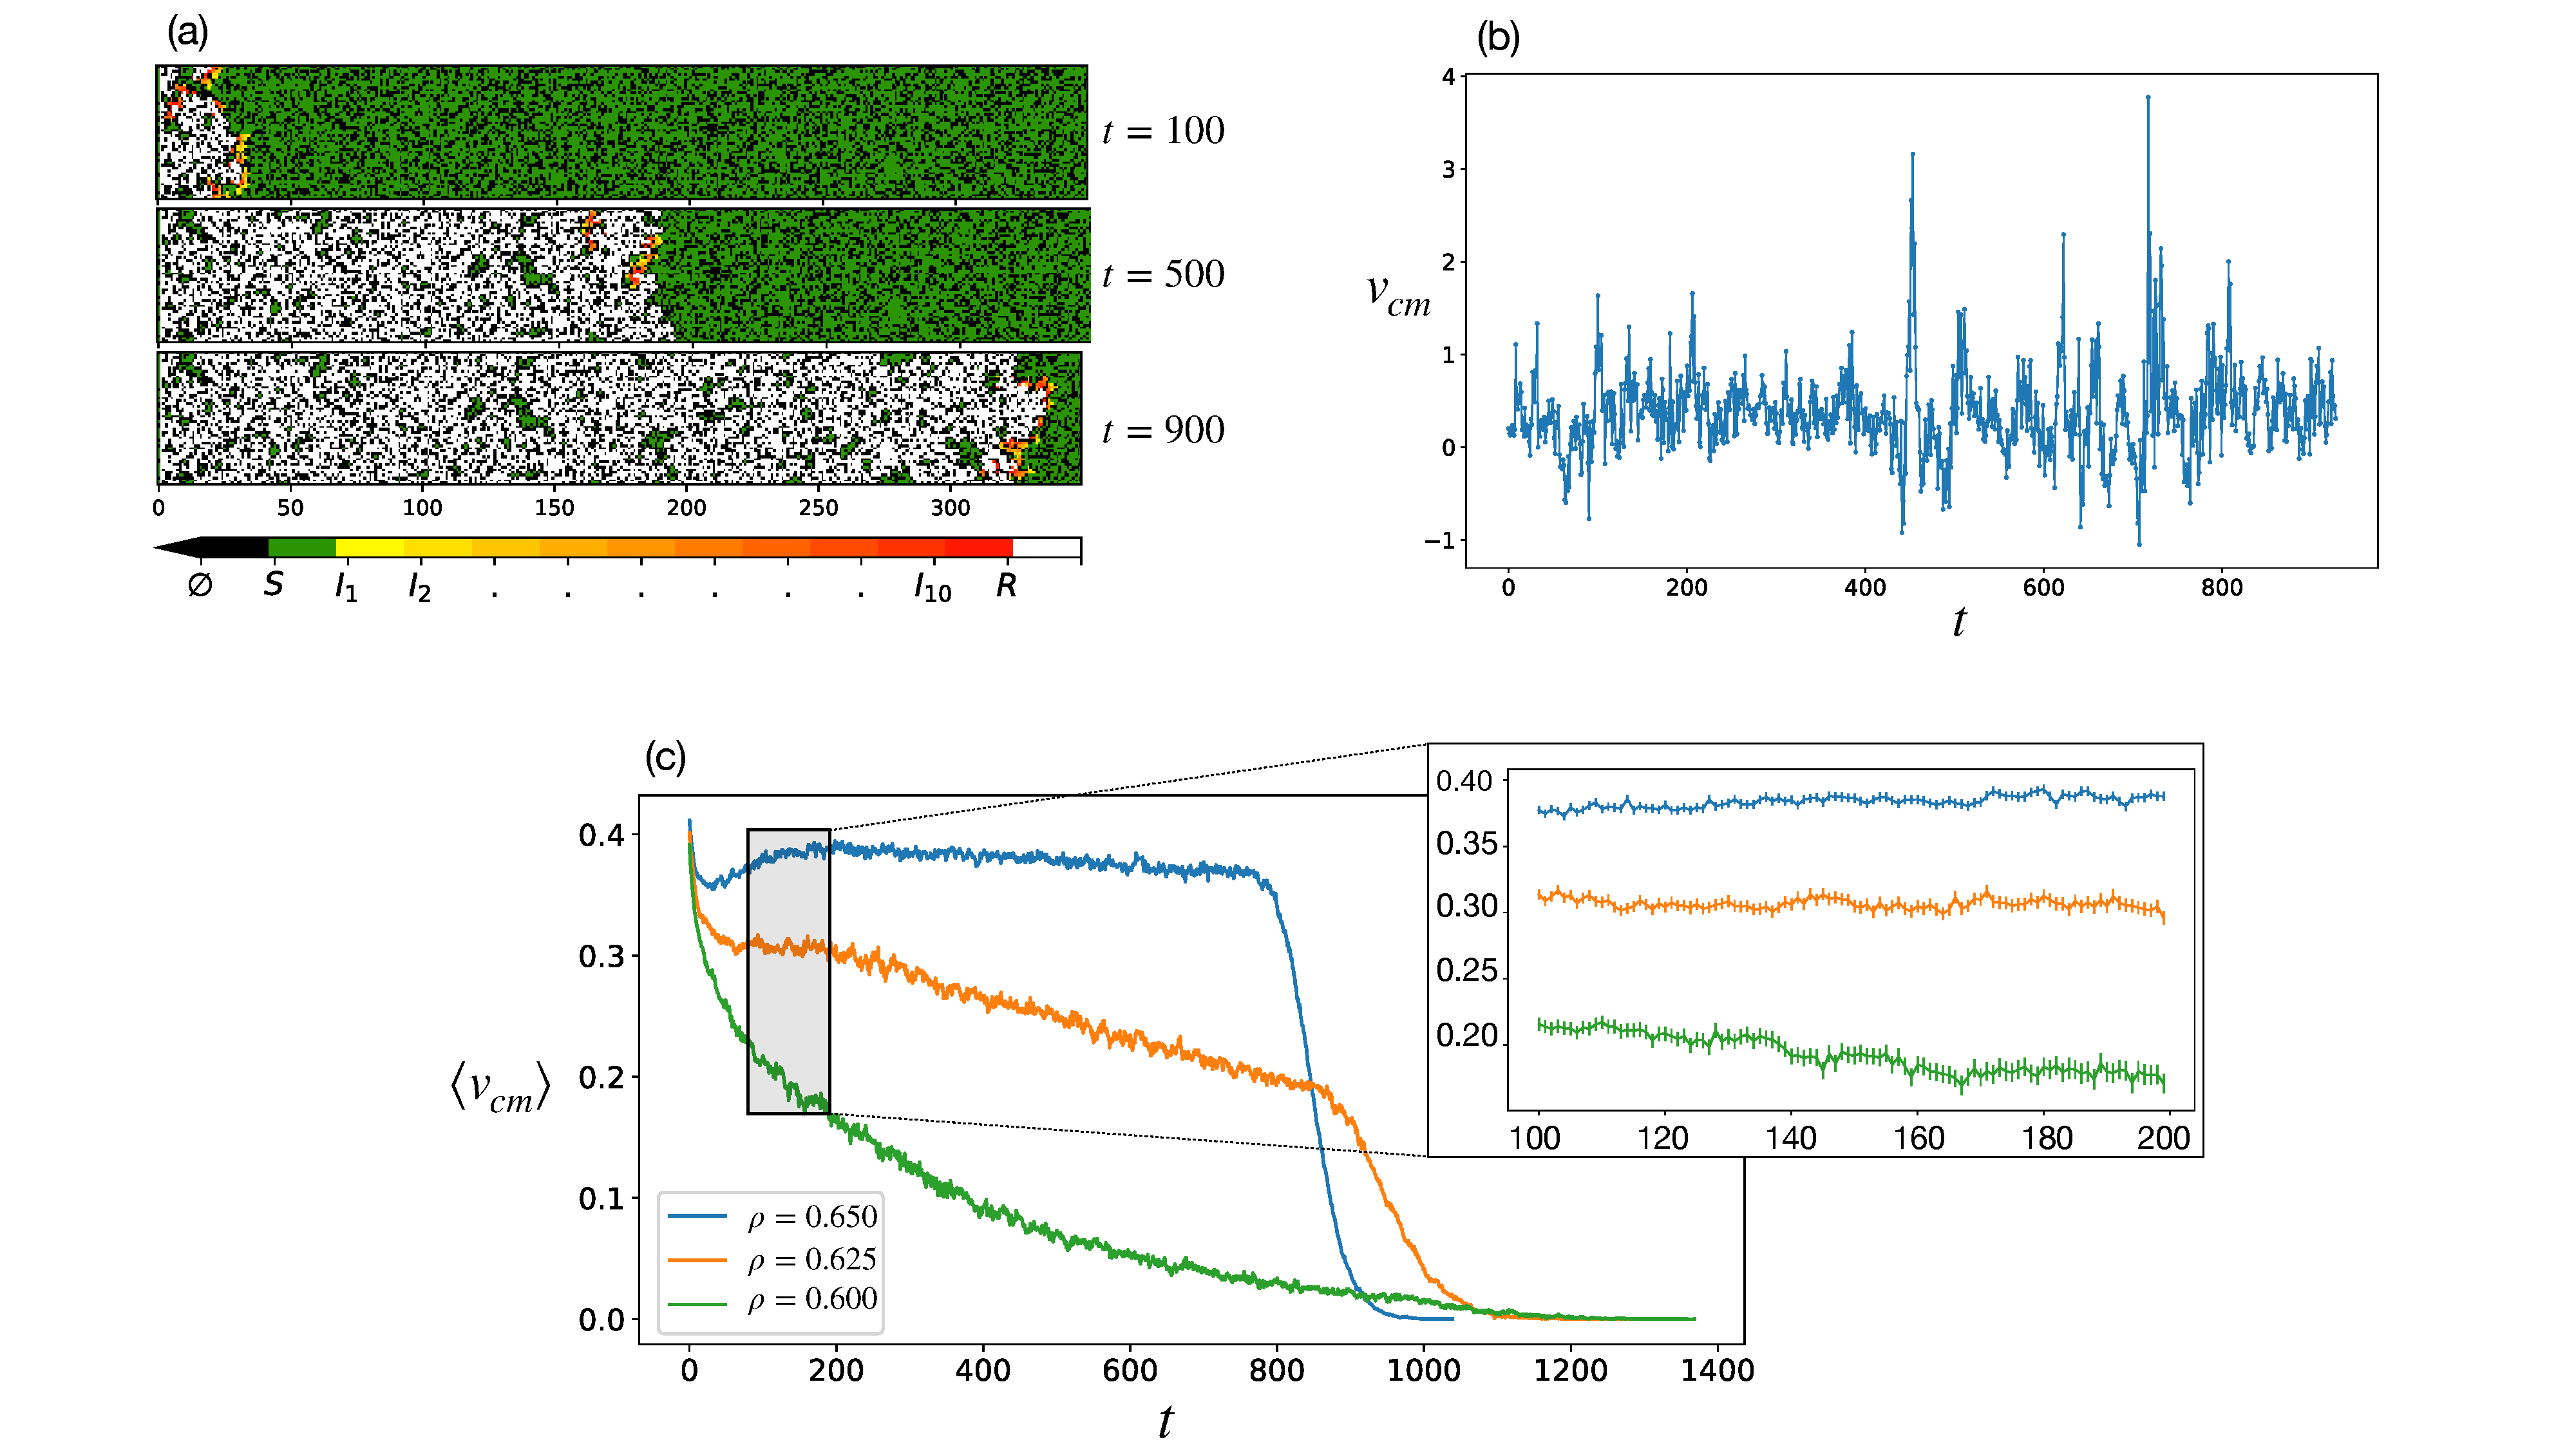
\includegraphics[scale=0.30]{chapter3/figures/figure10.pdf}
    \caption{(a) A channel domain of size $50\times350$ showing three time-steps of the model with parameters $\rho=0.65$ and $\beta=0.50$. The center of infectious mass is recorded for each time-step. (b) The center of mass time-series over the simulation. (c) The mean center of mass time-series (of $10^4$ repeats) for three variations in density and $\beta=0.50$. Time-series begin to decay around the mean simulation run-time.  The zoomed inset shows the ensemble averaged time-series for $t\in[100, 200]$ and reveals increases in error bars lower density parameters.}
    \label{fig:ews-primer}
\end{figure}

where $x_i(t)$ is the spatial location along the $x$ axis of the $ith$ infected tree at %
time $t$ and $N_I(t)$ is the total number of infected trees at time-step $t$. %
Comparing Eq (\ref{eq:COM}) with the Newtonian equation for center of mass: %
\begin{equation}
    x_{cm} = \frac{\sum^i x_i\times m_i}{\sum_i m_i}
\end{equation}
One can see the rate change in Eq (\ref{eq:COM}) can be considered as the `center-of-infection-mass' (COM) velocity %
with $m_i=1$ and $\sum^im_i= N_I$. %
This is easily implemented in Python, see Appendix \ref{a:slm_metrics}. %
The time-series of Figure \ref{fig:ews-primer}(a) is shown in Figure \ref{fig:ews-primer}(b) using $v_{cm}$. %
The COM time-series looks different to those shown previously in Figure \ref{fig:vel_eff_rad_metric}(a) allowing for the possibility of negative values. %

An ensemble average of the time-series, denoted by $\langle v_{cm}\rangle$ is illustrated in Figure \ref{fig:ews-primer}(c). %
Three different values of density were used and show  interesting properties: %
the mean time-series begins to systematically decay after the mean life-time of the simulation, %
the blue time-series shows a drastic decrease around $t \in [800, 900]$ when the pathogen %
reaches the boundary of the domain\textemdash illustrated in Figure \ref{fig:ews-primer}(a). %
The green time-series (being just above the threshold for percolation) decays gradually from %
the onset $t=0$ on account of a higher probability of extinction. %
A small number of long-lasting simulations $t>1000$ occurred in the green time-series and reflect criticalilty in the system. %

The inset of Figure \ref{fig:ews-primer}(c) shows the ensemble-averaged time-series between %
$t\in [100, 200]$ with the error measured for each time-step. Error bars, and therefore variance, %
is greatest for lower values of density, suggesting a more chaotic spread. %
In principle, if in-simulation variance such as this looks different before and %
after the epidemic regime is attained in parameter-space, an early warning signal could be detected. %

In general, a single simulation with parameters $\rho, \beta \in [0, 1]$ will last for $f$ time-steps. %
The metric-value at each step is defined Eq (\ref{eq:COM}) and can be described by the series, $v_{cm}^{t=1}, v_{cm}^{t=2},..., v_{cm}^{t=f} \in V^{\rho\beta}$. %
A set of independent time-series are generated by repeating $N$ simulations. %
A single point in the phase-space diagram is then described by $V_1^{\rho\beta}, V_2^{\rho \beta},..., V_N^{\rho\beta} \in \{\mathcal{V}_{\rho\beta}\}$, %
where $V_i^{\rho\beta}$ represents an arbitrary simulation time-series. %
Using this notation, an early warning signal is detected by calculating the mean time-series variance, %
defined by:
\begin{equation}
\label{eq:ews_eq}
    \big\langle \overline{var}(v^{\rho\beta}_{cm}) \big\rangle = \frac{1}{N}\sum\limits_{i=1}^{N} var(V_i^{\rho\beta})
\end{equation}

We proceed by detailing an ensemble-method that permits the capture of `in-simulation' variance. %

\subsection{Ensemble averaging method}

In order to properly analyse an ensemble of time-series variances, we require that the same %
number of observations are made within each ensemble. %
Otherwise, classification of an early warning signal might be confused and interpreted as %
a false positive\textemdash i.e. misjudged on account of statistical fluctuations and error. %
To ensure the number of observations are equal between all simulations, %
it is important to distinguish between a set of \textit{independent} simulations and the %
time-step observations which may differ between simulations. %

In general, any two independent simulations will not have the same number of time-steps, %
i.e. $|V_i^{\rho\beta}| \neq |V_j^{\rho\beta}|$. %
If this is not taken into account, comparisons between different ensembles will not be %
comparable because the variance calculated for short-lived simulations will be more error-prone %
than long-lived simulations. %
To remedy this, a fixed window of time-steps ($t_O\leq t \leq t_F$) is introduced. %
Provided the window length $t_F-t_O$ captures a sufficient number of time-steps, the effects %
of \textit{unlikely} large fluctuations in $V_i^{\rho\beta}$ are alleviated. Inside this window, %
the variance for all simulations will be calculated, Eq (\ref{eq:ews_eq}) is then slightly altered: %

\begin{equation}
\label{eq:ews_eq1}
    \big\langle \overline{var}(v^{\rho\beta}_{cm}) \big\rangle = \frac{1}{N}\sum\limits_{i=1}^{N} var(V_i^{\rho\beta}\Big|^{t_F}_{t_O})
\end{equation}

The precise choice of $t_O$ and $t_F$ is constrained by initial transience in the channel %
domain\textemdash analogously mentioned in the discussion of Figure \ref{fig:vel_eff_rad_metric}(a). %
Initial instability in the domain deserves some special consideration as it could distort %
calculations of the time-series variance. %
Figure \ref{fig:ews-primer}(c) reveals that transience occurs most for $t\in[0, 100]$, %
clearly demonstrated by increases in the blue time-series. %
The initial transience is less obvious for the blue and green time-series. %
As such, the first $100$ time-steps should not be included when calculating the variance. %
This means that all simulations that become extinct in less than $100$ time-steps are not %
included in the ensemble average. From these observations, the lower bound is valid for $t_O \geq 100$.%

Unfortunately, neglecting short-lived simulations $t<100$ introduces an additional complication. %
Namely, if we do not include these simulations, some ensembles $\mathcal{V}_{\rho\beta}$ %
(typically with low values of $\rho$ and $\beta$) will comprise less than $N$ measures of %
time-series variances. The ensemble mean, as calculated by Eq (\ref{eq:ews_eq}), will therefore %
be subject to more error which again could lead us to misclassify an early warning signal. %

An unbiased treatment of the ensemble thus requires i) the same number of time-steps in all %
simulations ii) the mitigation of initial instability iii) the same number of $N$ simulations %
are averaged for all points in phase-space. Combining all these requirements is clearly impossible %
for some points in parameter-space. Take the trivial example of $\rho=0$ and $\beta=0$, even %
as $N\rightarrow\infty$ not a single simulation will exist for $t\geq100$ steps and the %
variance remains undefined. For some fixed values of $\rho < \rho_c$ and $\beta<\beta_c$, %
the probability of all $N$ simulations surviving for longer than initial transience is zero. %

Fortunately, an early warning signal is only detectable immediately before and after the %
transition into an epidemic. If the \textit{mean} extinction time for these regions is %
above $t_F$, an early warning signal may be can be detected with confidence. %
Other regions in parameter-space well below-threshold are not important. %
So, a comparable treatment of ensembles can be accomplished provided that regions just %
below the point of epidemic-transition survive long enough to measure variance in the %
window $t \in [t_O, t_F]$. Should the value of $t_F$ be too large, a large proportion of %
simulations close, but below threshold, might not survive to give $N$ measures of variance. %

Given these concerns, a window was defined by setting the lower bound equal to the minimum %
value of $t_O=100$ and the upper bound to a value $t_F = 200$. %
These values were found to strike the best balance between: avoiding initial transience, %
ensuring that \textit{as many simulations as possible} on the verge of epidemic survive long %
enough to calculate variance and providing a sufficient window size. Using these conditions %
and the domain configuration of in Figure \ref{fig:ews-primer}(a), most simulations just below %
threshold (with some exceptions that are discussed below) were found to survive for longer %
than $200$ time-steps allowing for a multi-dimensional parameter-space analysis of early %
warning signals. %
 
\section{Early warning signal results}
\label{section:ews_slm}

Figure \ref{fig:ews-results} shows the mean time-series variance between $100\leq t \leq 200$. %
The value of variance is shown in the colour bar from white to black. %
The lower and upper red lines highlight regions in parameter space for which the %
probability of percolation is $Pr(\rho, \beta)=0.05$ and $Pr(\rho, \beta)=0.95$ respectively, %
those being the  critical regions in parameter-space that support an epidemic. %
The precise value of variance is not important, but crucially, a rise in time-series variance %
can be seen before the onset of epidemic. %
This is in agreement with the results found by \cite{OROZCOFUENTES201912}. %
%% with the benefit of being more adaptable to real-life time-series observations of tree diseases.

Assessing early warnings over a two-dimensional parameter-space reveals that some values %
of $\rho, \beta$ preempt the epidemic by a larger margin\textemdash indicated by the red %
arrows in Figure \ref{fig:ews-results}. Specifically this occurs for a lower infectivity %
($\beta<0.40$) and higher density. What aspect of the SLM gives rise to these differences %
behaviour when detecting an early warning signal? %

 \begin{figure}
    \centering
    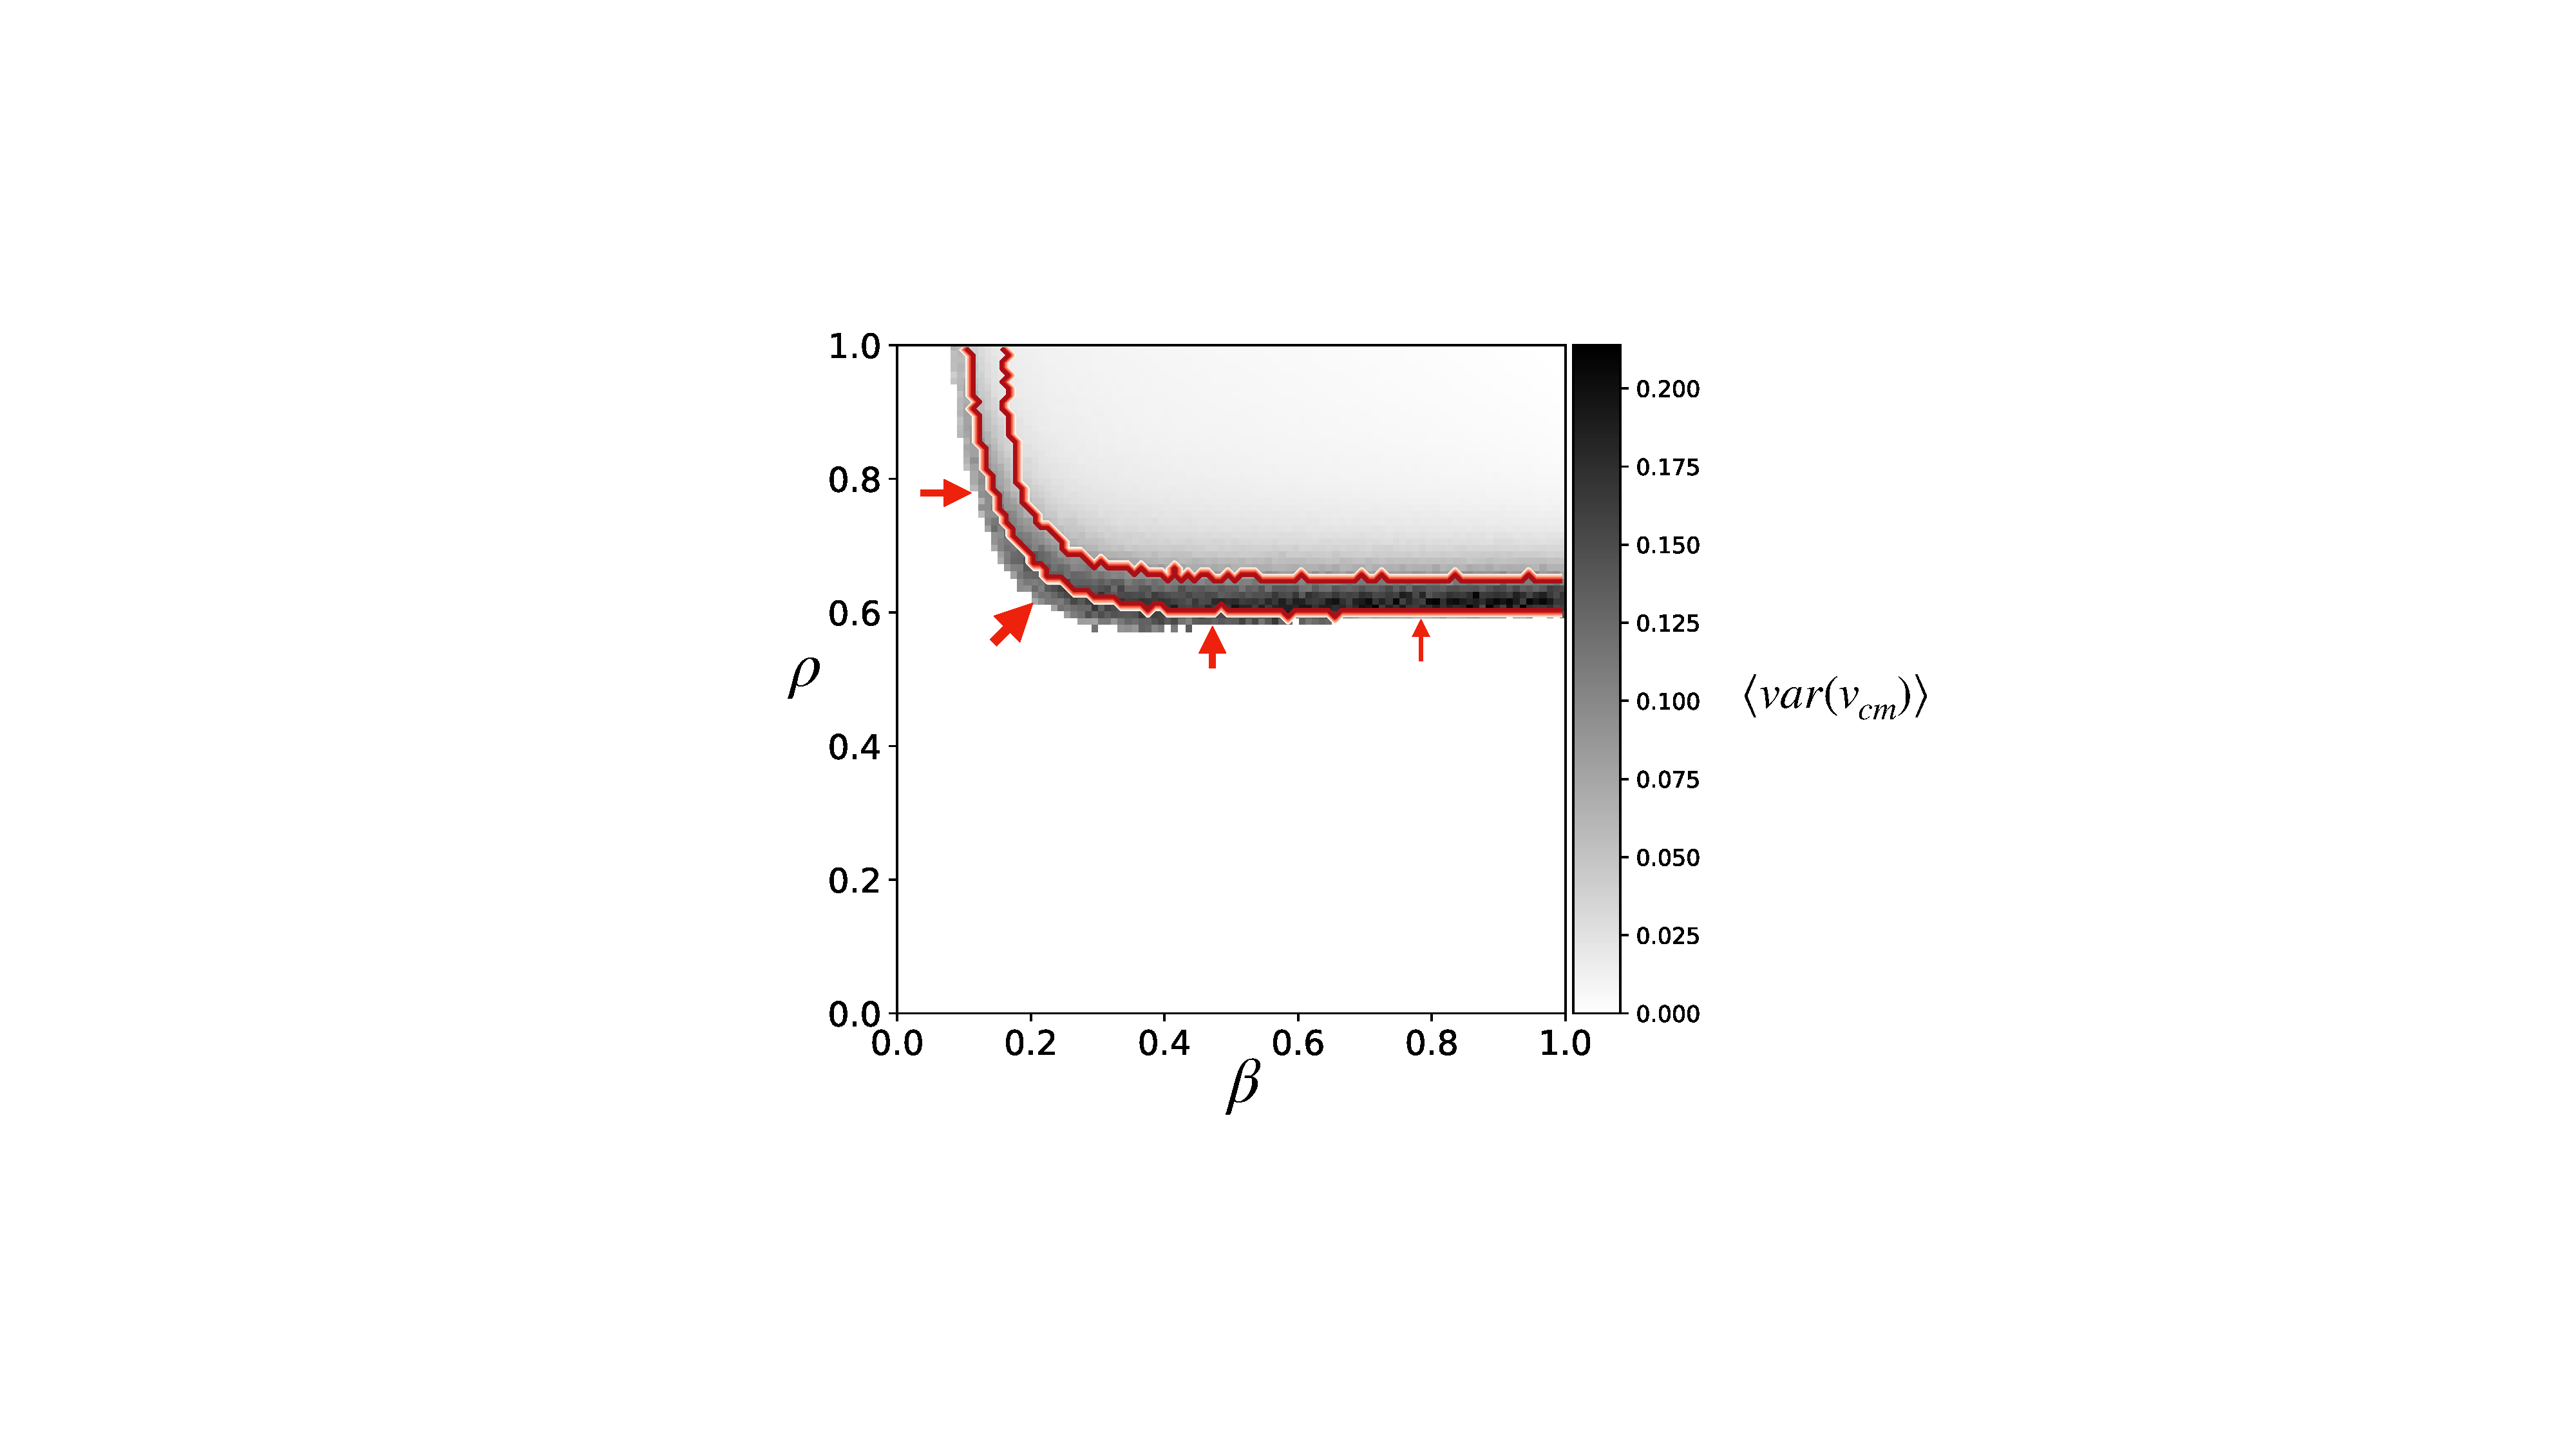
\includegraphics[scale=0.45]{chapter3/figures/figure11.pdf}
    \caption{The ensemble-averaged variance of $v_{cm}(t)$ over a two dimensional parameter sweep of $\rho$ and $\beta$. Red contours show the lower and upper bound of percolation (i.e. between $5\%$ and $95\%$ probability). 
     The epidemic regime is preempted by increases in variance more clearly for certain parameter values, %
     indicated by the arrows.}
    \label{fig:ews-results} 
\end{figure}


The asymmetry in early warning detection can be understood through the following thought-experiment: %
first, consider a high value of $\beta$ and density just below criticality $\rho\lesssim\rho_c$. %
In this case, the rate of disease progression is higher on account of $\beta$ and all hosts %
that are susceptible will become infected quickly. %
However, disease spread will soon come to a halt due to insufficient number ofhosts. %
An aggressive pathogen that has a low density of hosts will therefore propagate rapidly, %
have short extinction times and give rise to a more chaotic metric signature. %
Hence, the smallest arrow in Figure \ref{fig:ews-results} points toward a region where the %
variance spike is greatest and has no trace below the lowest bound of $5\%$ percolation probability. %

Conversely, a pathogen that has a low infectivity but an abundance of hosts will spread %
slowly but predictably through the domain. The pathogen is thus more likely to spread for a longer time before becoming extinct. In this scenario extinction times are long enough to process an early warning signal which precedes the epidemic by a larger margin, indicated by the large arrow(s) in Figure \ref{fig:ews-primer}. Here, variance can be seen to preempt the transition to a larger degree, however, the variance spike is not as strong.
 
These observations and Figure \ref{fig:ews-primer} point toward a distinction between an %
aggressive pathogen just below $\rho_c$ and a less aggressive pathogen well beyond $\rho_c$. %
 
%  \textcolor{red}{
%  \textbf{Notes}:
%  \begin{itemize}
%      \item I could add two additional sections for this Chapter:
%      \begin{enumerate}
%          \item The field equations as-per Rammiles derivation and simulate accordingly
%          \item The SLM running on a Voronoi lattice, which I did in first year but didn't take very far..
%      \end{enumerate}
%     \item These two points would in theory contribute to novelty of the project however, I see this as non-essential and something I can do at the end, if it comes to it
%  \end{itemize}}
 
\section{Chapter Summary}

This chapter started by introducing concepts from percolation theory. %
Firstly, percolation captured spatial stochasticity, given by the parameter $\rho$, on a regular square %
lattice with a homogeneous distribution of hosts. %
This was coupled to an $SIR$-based compartmental model along with a transmission dynamic. %
Connectivity between neighbours was defined by the Von Neumann neighborhood. %
The percolation threshold of this model was shown to be in agreement with the accepted value %
for a square lattice in two dimensions, $\rho_c = 0.593$. The nature of %
criticality was then considered with a short discussion on the  the universal properties of the model. %
Importantly, the universality and critical behaviour within the model was explained to supersede %
the particular geometry of a square lattice we have chosen. %   JS_What is the point you are making here?

Having established a one-parameter model based only on tree density $\rho$, a second parameter %
of infectivity $\beta$ was included. %
This parameter introduced a novel element of temporal stochasticity into the system %
and had large impacts on the speed of propagation. % JS_Be precise here.. too vague

Integrating infectivity into the model was justified given that pathogens display a range of %
pathogen-host interaction strengths. % JS_Did you discuss this with insight from your reading or was it speculation?
In general, interactions between hosts and pathogens are %
exceedingly complex % JS_this sounds like blah be more precise
and realistic descriptions should include many factors\textemdash % JS_give more details and prepare this properly
this is discussed in-depth when we move towards a non-local dispersal model in Chapter \ref{chapter:regional-containment}. %
For now, a simplified local model will suffice. %


The parallels between cluster-size and epidemic status are clear: % spell it out ore than this.
 an infinite cluster describes %
uncontrollable and infinite pathogen propagation. Clusters around $\rho_c$ describe a system %
on the verge of epidemic and sub-critical regimes describe systems below the epidemic threshold. %
In this model, a system below the threshold may sustain an outbreak for a time, but they will %
become extinct with certainty for some later time. %
Conceptually, this idea is described by the terminology `invasion' and `persistence' \cite{gilligan2008epidemiological}. %
%JS_ please be more precise
 
With the inclusion of infectivity $\beta$, we introduce the possibility that an outbreak will %
cease to spread even though the density of hosts is above criticality. %
That is, although an infinite cluster of connected hosts may be present,  %
stochasticity of transmission between infected and susceptible hosts may prevent infinite spread. %
Thus, a low value of $\beta$ acts to impede the spread of disease and makes it harder for a pathogen %
to propagate to the lattice-edge, as shown by Figure \ref{fig:slm_pspace}. %

The model we have defined %framed 
so far is representative of a forest, or nursery/plantation. %
The resolution of each lattice site is emblematic of the canopy cover assumed by a single tree, %
although for simplicity this was not defined. %
Additionally, the amount of time between steps in the simulations was left in arbitrary units %
along with the infectivity $\beta$. % JS_what are the alternatives?

What we have established in this chapter constitutes a simplified, abstract model of tree %
disease. Having laid the groundwork, we conveniently overlooked many important assumptions %
that include: 1) homogeneity within the lattice. 2) local interactions. 3) uniform %
transmission with equal probability $\beta$. 4) uniform transition rates into the $R$ compartment. %
5) arbitrary units and parameter values.  % JS_explain each of these further

Having established the SLM from first principles, the initial discussion of early warning %
signals conducted by \cite{OROZCOFUENTES201912} was revisited using an alternate framework. %
% 
We used the \textit{mean} time-series variance, opposed to the variance of the \textit{mean} %
time-series, a \textit{channel} domain with cylindrical boundary conditions and a metric that %
traced the center of infectious-mass over time. From this, we proceeded to capture early warning %
signals over a two dimensional parameter space whilst mitigating any unwanted geometrical effects. %
% JS_can you rewrite and explain this more carefully ?

When %setting up? 
defining the early warning framework, a detailed description of the ensemble-averaging process %
was given that permitted an unbiased treatment of simulations. %
In this way, early warnings %
were detected prior to the epidemic regime. Interestingly, asymmetries % JS_define these properly
in the detection of early %
 signals lead to some insightful observations about the model. %
 % JS_be clear what is insighful!
 Differences between a high $\beta$ and low $\rho$, were observed when compared against a low $\beta$ %
 and high $\rho$ regime. For a high $\beta$ and low $\rho$ regime, early warning signals were detected %
 further away from the epidemic regime. % JS_ explain further
 In contrast, early warning signals for a low $\beta$ and high $\rho$ regime were only %
 observable immediately before epidemic transition, although the variance spike was larger. %

From these findings we may conjecture how it would be easier or harder to detect and prevent %
either: a pathogen with infectivity on the verge of epidemic, or a region of hosts just below %
the critical density. % JS_How dow these comment help you interpret other research?
This could apply to a variety of systems in which environmental factors act to tip the pathogen %
spread over the threshold for epidemic. % % JS_Can you explain what they are?

Problematically however, the spread of disease through real systems cannot be ensemble averaged. %
It therefore remains a speculative matter to consider how applicable this framework could be to %
real landscapes and pathological systems. Early warning signals would be hard to resolve accurately in %
practice due to various factors, including the cryptic nature of infestations, %
long-ranged dispersal and more generally an insufficient knowledge of infected symptomatic hosts. %
This re-investigation thus remains abstract and more work would need to be conducted before %
accurate results can be established. %

\newpage